\documentclass[11pt,a4paper]{article}

% Text- und Font-Encoding:
\usepackage[utf8]{inputenc}
\usepackage[T1]{fontenc}

% Worttrennung auf Deutsch:
\usepackage[ngerman]{babel}

\usepackage{listings}

\pagestyle{headings}

% Zeilenabstand
\usepackage{setspace}
\setstretch{1.3}

% Captions
\usepackage[labelsep=newline,labelfont=bf,figurename=Abb.]{caption}
\usepackage{subcaption}
\usepackage[pdftex]{graphicx}

\usepackage{acronym}

% Präambel ende

\begin{document} 


\begin{titlepage}
	\centering
	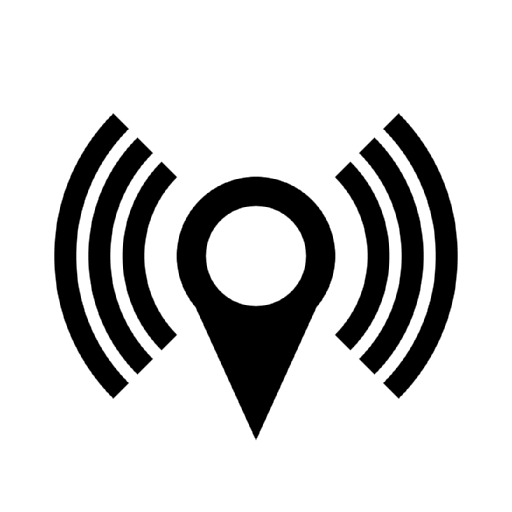
\includegraphics[width=0.25\textwidth]{pics/airsniffer.png}\par\vspace{1cm}
	{\scshape\LARGE Hochschule für Technik und Wirtschaft Berlin \par}
	\vspace{1cm}
	{\scshape\Large Independent Coursework\par}
	\vspace{1.5cm}
	{\huge\bfseries Erfassung und Verarbeitung von WLAN Signalen anhand von mobilen Endgeräten für die Nutzung als Positionierungssystem\par}
	\vspace{2cm}
	{\Large\itshape Fabian Bänsch\par}
	\vfill
	betreut von\par
	Prof. Dr. Gefei \textsc{Zhang}

	\vfill

% Bottom of the page
	{\large \today\par}
\end{titlepage}

\tableofcontents{}

\newpage

\section{Vorstellung}

Diese Arbeit dient als Dokumentation und Erklärung des Independent Courseworks zum Thema "Erfassung und Verarbeitung von WLAN Signalen anhand von mobilen Endgeräten für die Nutzung als Positionierungssystem".

Dieses Verfahren zur Positionsbestimmung mittels WLAN Signalen wird bereits angewandt. Jedoch sind die bisherigen Crowdbasierten Ansätze für die Erstellung solch einer Plattform zu gering vertreten und schwach verbreitet. Die Arbeit soll daher prototyptechnisch diese Thematik untersuchen und am Ende evaluieren.

Es werden dabei verschiedene Softwarekomponenten auf verschiedenen Plattformen für die jeweiligen Aufgaben erstellt. Es wird dabei nur oberflächlich auf die Implementierung eingegangen. Sämtlicher Sourcecode Code ist auf GitHub~\cite{github} veröffentlicht. 

\section{Konzept}

Mit der Öffnung des Global Positioning Systems~(GPS)~\cite{gps} im Jahre 2000 für die zivile Nutzung war es erstmals für den Endanwender möglich eine Lokalisierung mit einfachen technischen Geräten wie Smartphones zu erreichen.

Das GPS besteht dabei aus einer Reihe an geostationären Satelliten, welche permanent codierte Radiosignale an die Erde senden. Darin sind der Standort des Satelliten und die genaue Uhrzeit enthalten. Empfangsgeräte können aus diesen Signalen dann ihren Standort mittels der Signallaufzeit errechnen. Eine Sichtverbindung zu mindestens 4 Satelliten wird benötigt.

Dieser Prozess kann entsprechend lange dauern. Das Phänomen wird umgangssprachlich auch "GPS Fix" genannt~\cite{gpsfix}. Also die verstrichene Zeit, bis das GPS Signal so stabil ist, dass eine Berechnung erfolgen kann. 

Zum anderen hat das globale Positionierungssystem auch Schwächen in stark urbanisierten Bereichen. So ist in Großstädten mit hohen Häusern die Genauigkeit der Berechnung der Position eher schlecht. Dies ist zum einen durch die Verdeckung von Satelliten mit Hochhäusern zu erklären, anderseits kann es auch auch zu Reklektionen von GPS Signalen führen, welche die Positionierung verschlechtern.

Die Idee hinter der WLAN-basierten Ortung gibt es schon bereits seit längerem. Hierbei können Geräte die sichtbaren WLAN Netze in ihrer Umgebung an einen zentralen Service senden. Dieser Service kann durch eine Verknüpfung von WLAN Netz und Position des Netzes, den Standort des Anfragers errechnen. Dazu muss jedoch der Service über die entsprechenden Daten verfügen. Das heißt, zu sämtlichen Netzen muss der Standort gespeichert sein. Der Aufbau dieser Datenbank stellt dabei eine Sisyphusarbeit dar und muss regelmäßig überholt werden. Anbieter wie Skyhook~\cite{skyhook} oder Google~\cite{google_pos} nutzen dazu spezielle Fahrzeuge mit Messantennen, welche durch die Städte fahren (meist in Verbindung mit anderen Aufgaben). 

Daneben gibt es auch solche Services, welche auf Crowdbasierte Informationen zurückgreifen. Dabei kann jeder einen Beitrag leisten und so zum Aufbau, Erweiterung und Wartung des Services beitragen. Als Beispiel seien hier Wigle~\cite{wigle} oder OpenWifi.su.~\cite{openwifi} genannt.

Als primärer Verwendungszweck des hier vorgestellten Projekts soll eben dieser Crowd-basierte Ansatz sein.

Im weiteren Verlauf der Arbeit wird daher zunächst noch einmal ein Blick auf raumbezogene Daten geworfen und inwiefern diese verarbeitet werden können. Danach folgt eine allgemeiner Abriss über das Anwendungsdesign und aller Komponenten des Systems. 

In den folgenden Kapiteln wird dann zunächst erläutert wie WLAN Daten gesammelt werden, diesen dann einer zentralen Einheit (API) zugestellt werden und mittels einer Visualisierung bzw. der Standortbestimmung seitens des Endanwenders benutzt werden kann.

%TODO Warchalking

\section{Geospatial Data}

Dieses Kapitel gibt eine kurze Einführung in raumbezogene Daten, wie mit dieses gerechnet werden kann und wie eine Interpolation für das hier vorgestellte System durchgeführt wird.

Raumbezogene Daten auf der Erde können auf verschiedenen Arten angegeben werden. Hierbei wird die Erde als Kugel betrachtet und entsprechend können Kugelkoordinaten als Ortsbestimmung benutzt werden. Dazu werden 180 Breitengrade (horizontal) und 360 Längengrade (vertikale) erstellt. Ein Punkt auf der Erde kann nun mit nur 2 Angaben eindeutig bestimmt werden. Der speziellen Längen und Breitengrade. Klassischerweise wird dabei zu Verfeinerung mit Stunden, Minuten und Sekunden gearbeitet. Da Computer eher schlecht ein Basis 60 System zu Berechnung nutzen können, kann die Unterteilung auch dezimal erfolgen. Dies wird hier auch der Fall sein. 

Um die Distanz von 2 Punkten berechnen zu können wird die harversine Distanz verwendet. Sie stellt sicher, dass die Krümmung der Erde bei der Distanzberechnung mit berücksichtigt wird~\cite{harversine_distance}.

\begin{lstlisting}[language=Java]
public static final double R = 6372.8; // In kilometers
public static double haversine(
		double lat1, 
		double lon1, 
		double lat2, 
		double lon2) {
    double dLat = Math.toRadians(lat2 - lat1);
    double dLon = Math.toRadians(lon2 - lon1);
    lat1 = Math.toRadians(lat1);
    lat2 = Math.toRadians(lat2);
    double a = Math.pow(Math.sin(dLat / 2),2) +
    	Math.pow(Math.sin(dLon / 2),2) * 
    	Math.cos(lat1) * Math.cos(lat2);
    double c = 2 * Math.asin(Math.sqrt(a));
    return R * c;
}
\end{lstlisting}

Da wir später an mehreren Orten das WLAN Signal eines Routers einfangen werden, stellt sich die Frage, wie können wir auf den Quellort des Signals schließen? Hier gibt es mehrere Verfahren. Ich werde zu Beginn lediglich den Durchschnitt der Koordinaten als Zentrum benutzen. In späteren Versionen kann dort noch ein Gewichtung mit der Qualität des GPS und der aktuellen Empfangsleistung des WLAN kombiniert werden.

\section{Anwendungsdesign}

Das System wird sich wie eingangs erwähnt in 4 Teile untergliedern, welche voneinander teilweise losgelöst arbeiten können.

Der ''\textbf{AirSniffer}'' ist die Smartphone Anwendung, welche für das Sammeln der Daten zuständig ist. Diese muss dabei so gestaltet werden, dass zunächst keine API Anbindung notwendig ist. Sie soll autark - also offline - ebenso funktionieren. Daher muss hier eine Datenbank zur Speicherung der lokalen Ergebnisse stattfinden. Diese Resultate können dann an die API gesendet werden, um die Daten zu veröffentlichen. Als Prototyp wird eine Anwendung in Android (nativ) umgesetzt. 

Die ''\textbf{AirPI}'' dient als zentraler Service des Systems. Hier können die Daten der AirSniffer App hochgeladen werden. Zudem werden Funktionalitäten zum Abrufen der WLAN bzw. raumgebundenen Daten angeboten, welche die verarbeitenden Apps nutzen können. Die API wird unter Python mit Flask~\cite{flask} laufen. Für den Datenhaushalt sorgt eine MongoDB~\cite{mongodb}.

Die ''\textbf{AirVis}'' Anwendung dient als Visualisierungstool der Daten aus der AirPI. Die webbasierte Anwendung stellt dabei eine interaktive Karte mit verschiedenen Filterfunktion zur Verfügung. Daraus können aus den Rohinformation ein umfangreicher Mehrwert gezogen werden. Technologien für die Umsetzung sind dabei HTML, Javascript und CSS. Zudem wird die Google Maps API~\cite{googlemapsapi} verwendet. Aufgesetzt wird die Anwendung in einer Linux / Apache Umgebung.

Der ''\textbf{AirLocator}'' ist eine beispielhafte Anwendung, welche auf Grundlage der Daten aus der API eine Positionsbestimmung durchführt. Die eigentliche Berechnung wird dabei von der AirPI ausgeführt. Die Anwendung dient lediglich als Anzeige. Wie auch der AitSniffer wird sie als native Android API mit einer Google Maps API Anbindung programmiert.

Alle Komponenten in ihren Beziehungen sind in Abbildung~\ref{fig:Anwendungsdesign} ersichtlich.

\begin{figure}[htbp]
    \centering
    \begin{subfigure}[b]{1\textwidth}
        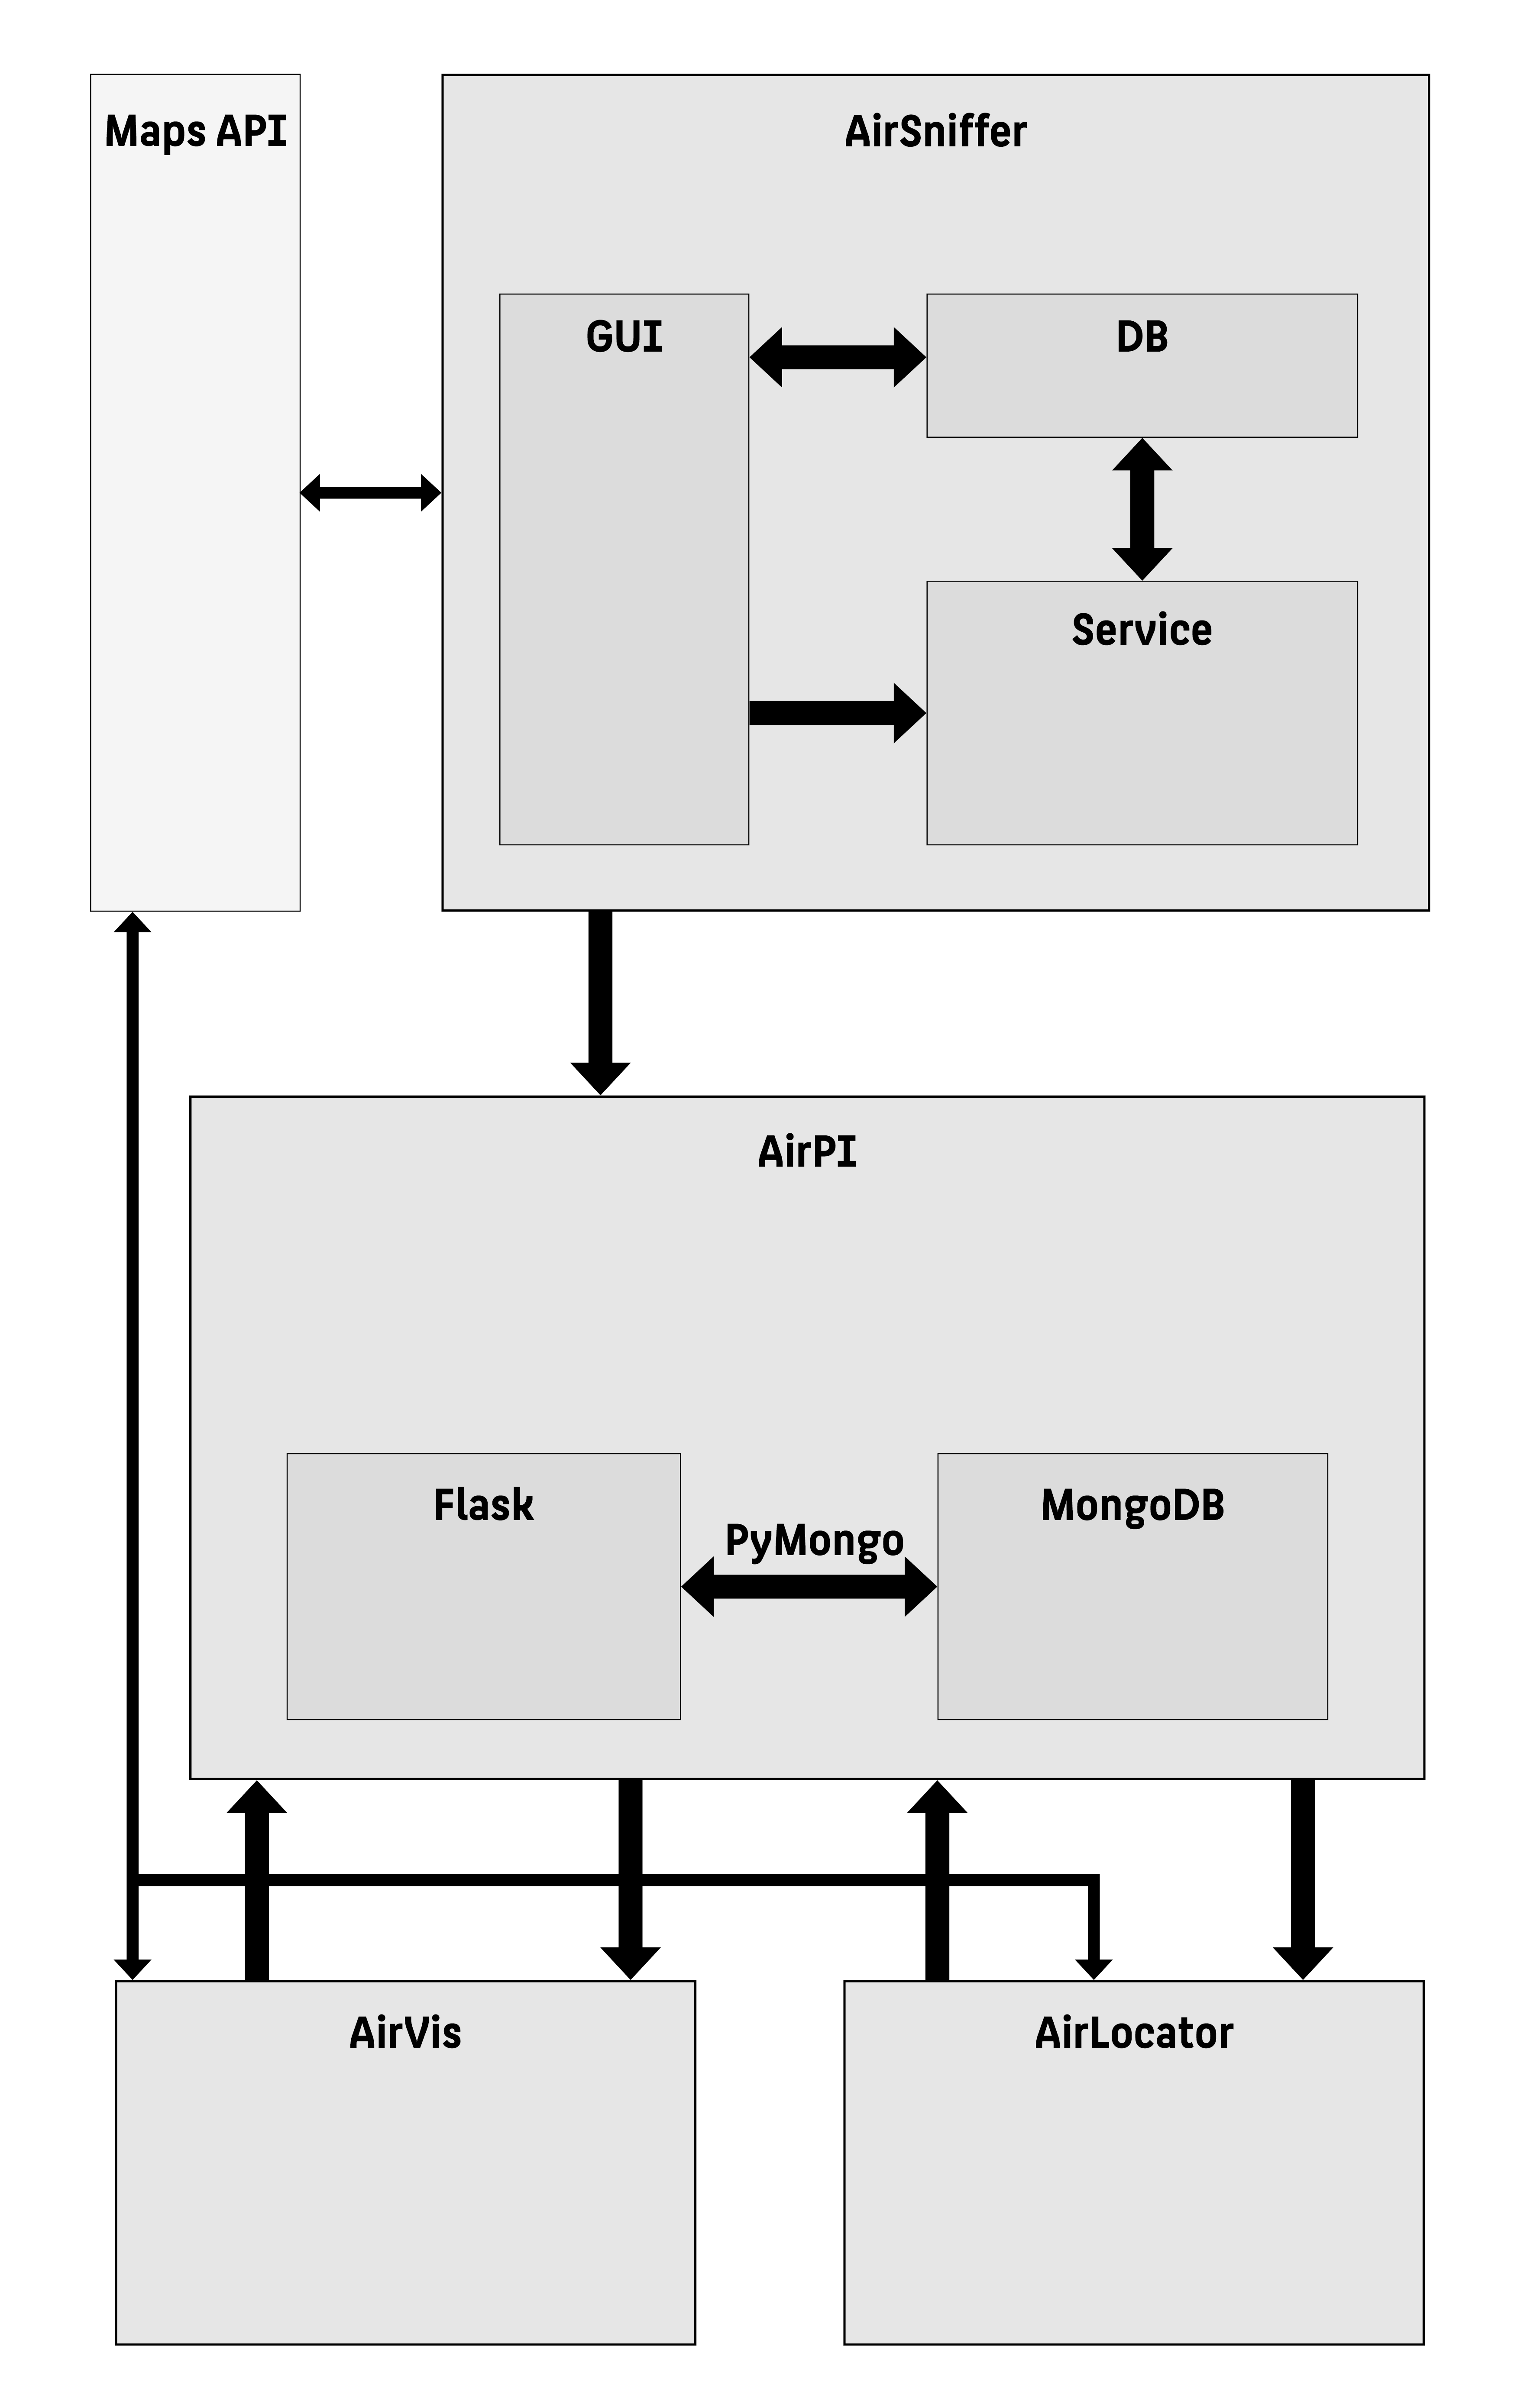
\includegraphics[width=\textwidth]{pics/AirAndwenungsdesign.png}
    \end{subfigure}
    \caption{Anwendungsdesign}\label{fig:Anwendungsdesign}
\end{figure}

\newpage
\section{AirSniffer}

Als Datenerfassungsandwendung wurde wie eingangs der AirSniffer entwickelt. Dies ist eine App unter Android. Sie soll dabei autark von der API bereits laufen können, und ähnliche Funktionalitäten aufweisen. Dazu musste zunächst eine Datenbank auf dem Endgerät erstellt werden, um die aufgespürten Netzwerke persistent abzuspeichern. Android bietet dazu eine relationale SQLite~\cite{sqlite} Datenbank an. Für den Anwendungsfall hier haben dabei 2 Tabellen gereicht. Eine für die WLANs und eine zur Speicherung der Örtlichkeit. Dabei entsteht eine 1:n Beziehung. Das heißt, ein Gerät kann mehrere Örtlichkeiten haben. Die Örtlichkeiten stellen dabei die Orte dar, an dem das Netzwerk sichtbar war. Die  Struktur der Datenbank sieht entsprechend wie folgt aus~\footnote{Die Datenbank weißt teilweise auch Felder auf, welche nicht speziell in dieser Arbeit vorgestellt werden.}

\begin{figure}[htbp]
    \centering
    \begin{subfigure}[b]{1\textwidth}
        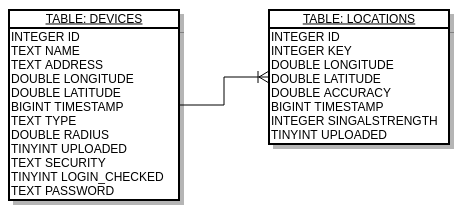
\includegraphics[width=\textwidth]{pics/dbView.png}
    \end{subfigure}
    \caption{Datenbankmodell}\label{fig:DB_VIEW}
\end{figure}

Der Key aus der ''Locations'' Tabelle dient dabei als Fremdschlüssel für den Eintrag aus ''Devices''. Jeder ''Device'' Eintrag hat zudem selber ein Feld mit der Angabe zur Längen- und Breitengrad. Hier wird später der Mittelwert errechnet und eingetragen. Dies dient lediglich der Perfomancesteigerung. 

Um das Protokollieren von WLAN Daten im Hintergrund ausführen zu können, wurde eine selbständiger Service implementiert. Dieser ist unabhängig von der App. Die App mit den GUI (Graphical User Interface) Elementen kann diesen lediglich starten und stoppen. Daraus ergeben sich jedoch auch folgende Vorteile: Der Background Service erhält mehr Rechenleistung und er kann auch bei nichtaktiver GUI weiterarbeiten. Der wichtigster Vorteil ist jedoch, dass der Service nicht abbrechbar seitens Android ist. Normalerweise unterbricht Android nebenläufige Hintergrundprozesse nach einer gewissen Zeit. Ebenso kann der Prozess auch nicht beendet werden, wenn der Benutzter die App (GUI) absichtlich versucht zu stoppen. 

Nachteilig ist jedoch, dass die Kommunikation von GUI und Backgroundservice nicht mehr einfach herzustellen ist. Daher wurde für GUI Anwendung lediglich auf die Einträge der Datenbank zurückgegriffen.

Das Mitlesen der Nachrichten findet nun im Backgroundservice statt. Hier können verschiedene Sniffer Instanzen gestartet werden
\footnote{Es gibt Sniffer für WLAN Netze, Bluetooth Low Energy Geräte und Bluetooth EDR Geräte. Hier in der Arbeit wird primär auf den Einsatz der WLAN Netze eingegangen}.
Das Mitlesen von derzeitig verfügbaren WLAN Netzen unter Android kann wie im folgenden Codebeispiel angeregt werden.

\begin{lstlisting}[language=Java]
String connectivityContext = Context.WIFI_SERVICE;
final WifiManager wifiManager = (WifiManager) getContext()
   .getSystemService(connectivityContext);
if (wifiManager.isWifiEnabled()) {
   wifiManager.startScan();
}
\end{lstlisting}

Die Callbacks werden typischerweise unter Android mit einem Broadcastreceiver aufgefangen. Notwendiger müssen diese zunächst angemeldet werden. Ein beispielhafter Broadcastreceiver sieht wie im folgenden Codebeispiel aus:

\begin{lstlisting}[language=Java]
BroadcastReceiver receiver = new BroadcastReceiver() {
   @Override
   public void onReceive(Context context, Intent i) {
      WifiManager wm = (WifiManager) context
      .getSystemService(Context.WIFI_SERVICE);
      List<ScanResult> results = wm.getScanResults();
      for (ScanResult scanResult : results) {
         String ssid = scanResult.SSID;
      }
   }
};
\end{lstlisting}

Diese Scanresults werden dann adaptiert auf das ''Device'' Modell und zusätzlich mit den aktuellen Koordinaten versehen. Um die Performance zu steigern wurde auch eine Senke als Thread erstellt, welche für das weitere Handling zuständig ist. Hier wird beim Versuch das neue Geräte der Datenbank hinzuzufügen zunächst geschaut, ob es bereits enthalten ist. Ist dies der Fall, so werden lediglich die neuen Koordinaten als weiteren Ort hinzugefügt
\footnote{Dabei werden noch weitere Berechnungen durchgeführt. Zum Beispiel muss ein Mindestabstand von 2m zwischen verschiedenen Orten gewährleistet sein. Es werden zusätzlich die Daten auf Richtigkeit geprüft. So ist ein sehr schlechtes GPS Signal zum Beispiel nicht weiter verwendbar und der Eintag wird verworfen}.
Im Folgenden weiteren weitere Information hinzugefügt. So wird einer neuer Mittelpunkt des Netzes sowie sein Radius berechnet. Im Falle eines neu entdeckten Netzes wird auch eine Notification samt Vibration an das Android OS gesendet (siehe Abbildung~\ref{fig:AirSniffer_Notification}).

Die eigentliche App mit sämtlichen GUI Elementen ist wie oben beschrieben unabhängig von dem eigentlichen Sniffen. Hier gibt es verschiedene Views, welche auch teilweise die Google Maps API~\cite{googlemapsapi} verwenden.
So gibt es zunächst eine Listenansicht mit allen lokal gesnifften Netzen (siehe Abbildung~\ref{fig:AirSniffer_Home_List}). 
Ein Indikator gibt an, ob es sich um ein WLAN, BL LE oder BL EDR Gerät handelt. Zudem kann man auch direkt nach Netzen suchen. Die Detailansicht eines Gerätes offenbart zusätzlich alle referenzierte Orte, an den das Gerät sichtbar war (siehe Abbildung~\ref{fig:AirSniffer_Detail_List}). 
Beide Views können dabei auch als Kartenansicht gestartet werden. Dabei wird zum Beispiel auch der Radius visualisiert 
(siehe Abbildungen~\ref{fig:AirSniffer_Home_Map} \& \ref{fig:AirSniffer_Detail_Map}). Sämtliche Informationen sind jedoch lokal erstellt und stammen vom eigenem Gerät. Daher stellt die Anwendung auch eine Logik zum Hochladen sämtlicher gesnifften Netze an die AirPI zur Verfügung. Hierbei wird auf das Json Format zurückgegriffen. 

Es hat sich unter Android gezeigt, dass es keine Suche nach WLAN Netzen seitens des Betriebssystems gibt, wenn der Bildschirm in den Ruhezustand geht. Daher wurde eine zusätzliche View erstellt, welche als Sperrbildschirm dient und den Bildschirm nicht abschaltet (siehe Abbildung~~\ref{fig:AirSniffer_Lockscreen}).

%TODO wificracker anteasern

\section{AirPI}

Dieser Teil des Systems soll als zentrales Rückgrat dienen. Hier können ersniffte Netze hochgeladen und gespeichert werden. Zudem sollen weitere Prozeduren enthalten sein, um diese zu optimieren und zu validieren. 
Des weiteren sollen Schnittstellen gefunden werden, um die vorhanden Daten sinnvoll  verschiedene Services anzubieten.

Technisch wurde hier aus einer Kombination von Flask~\cite{flask} und MongoDB~\cite{mongodb} mit PyMongo~\cite{pymongo} als Bindeglied gesetzt. Flask ist ein Webframework unter Python. Enthalten ist eine Template Engine ''Jinja2'' und die hier benötigte Bibliothek ''Werkzeug'' zum erstellen von WSGI Anwendungen (Web Server Gateway Interface). Flask ist sehr handlich. Die Hello World Anwendung besteht aus gerade mal 7 Zeilen Code~\cite{flask}.

\begin{lstlisting}[language=Python]
from flask import Flask
app = Flask(__name__)

@app.route("/")
def hello():
    return "Hello World!"
    
if __name__ == "__main__":
    app.run()
\end{lstlisting}

\noindent Zusätliche wurde eine Basic Authentifizierung eingeführt. Diese ist mit einem statischen Benutzer und Kennwort vorgegeben.
Mit dieser Vorgehensweise wurden folgende API Signaturen erstellt. 

\begin{lstlisting}[]
GET     /devices
POST	/devices
GET     /devicesAtPos
GET     /devicesAtRect
GET     /device
GET     /status
GET     /alive
POST    /location
\end{lstlisting}

Die MongoDB Datenbank ist eine Dokumentbasierte Datenbank. Daher kann die relationale Datenbank aus Android nicht einfach auf diese gemappt werden. Stattdessen ist nun die ''Locations'' Tabelle, welche via Fremdschlüssel angesprochen wurde, direkt als Set im ''Device'' Modell enthalten. Dies stellt auch automatisch sicher, dass keine Duplikate von Orten enthalten sein können.

Die MongoDB wird nicht direkt angesprochen, sondern mit den PyMongo Wrapper. Hier lassen sich nach erfolgreichen Instanzierung aber auch normale MongoDB Queries starten. Beispielhaft sieht das wie im folgenden Codebeispiel aus:

\begin{lstlisting}[language=Python]
from flask_pymongo import PyMongo
app.config['MONGO_DBaddress'] = 'db'
app.config['MONGO_URI'] = 'mongodb://localhost:27017/db'
mongo = PyMongo(app)
devices = mongo.db.devices.find()
for device in devices:
   app.logger.info(str(device))
\end{lstlisting}

Hier werden lediglich alle ''Devices'' aus der Datenbank geladen und via dem Logger ausgegeben. 
Ein großer Vorteil von MongoDB ist das Arbeiten mit dem Geospatial-Index, welcher direkt angeboten wird. Dadurch kann die MongoDB höchstperfomant eine Reihe an Daten liefern, welche zum Beispiel innerhalb einer gegebenen Bounding Box liegen. Dazu ein Codebeispiel:

\begin{lstlisting}[language=Python]
mongo.db.devices.create_index([("loc", GEO2D)])
query = [{"loc": {"$within": {"$box": [
   [swLon, swLat], [neLon, neLat]]
   }}}]
devices = mongo.db.devices.find({"$and": query}
\end{lstlisting}

\newpage
\noindent
Im folgenden werden einige Routen mit deren Funktionalitäten vorgestellt.

\begin{itemize}
\item{} \textbf{GET /devices}

Hier werden alle Devices geliefert, welche den Typen aus der Parameterliste übereinstimmen. Diese Route ist nur für Testzwecke und für die Anbindung an andere Services gedacht. 
%TODO welche Services - dieses github dingens?!

\item{} \textbf{POST /devices}

Das Hinzufügen von neuen Geräten aus der AirSniffer Applikation wird über diese Route gehandhabt. Die entsprechenden Geräte müssen im Body des Requests als Json vorliegen. Im Nachhinein findet noch eine Optimierung satt. Das bedeutet, zu nah aneinander liegende Orte werden entfernt sowie der Berechnung von einem neuen Mittelpunkt und dem Radius.

\item{} \textbf{GET /devicesAtPos}

Mittels des Geospatial-Index werden hier alle Geräte geliefert, welche an einem Ort und deren Umkreis liegen. Diese Daten werden als Query Parameter mit übergeben.

\item{} \textbf{GET /devicesAtRect}

Ähnlich der vorherigen Route. Nur kann hier eine Bounding Box angegeben werden.

\item{} \textbf{GET /device}

Weitere Informationen zu einem Gerät inklusive aller vorhanden Orte bei denen das Gerät erkundet wurde, werden hier geliefert. Als Identifikationsmittel wird die MAC Adresse des Gerätes via Query Parameter mit hineingereicht.

\item{} \textbf{POST /location}

Diese Route berechnet anhand von gegeben MAC Adressen den mittleren Standort. Die Adressen werden im Request Body als Json mit übergeben. Anhand des mittleren Standorts der Geräte kann im folgenden eine Positionsbestimmung eines Clients durchgeführt werden. Abbildung~\ref{fig:ScreenShot_AirPI} zeigt einen beispielhaften Request an die AirPI mit den WLAN Daten und den entsprechenden Response mit der errechneten Position.

\end{itemize}

%TODO Dependencies
%TODO Installationsanleitung
%TODO Beispiel GET mit Request

\section{AirVis}

AirVis ist die Visualisierungskomponente in diesem System. Sie ist webbasiert und ermöglicht die Veranschaulichung der in der AirPI gespeichert Daten. Durch das einfache Navigieren mittels einer Karte und verschiedenen Filterungstechniken entsteht ein erheblicher Mehrwert für den Nutzer. Abbildung~\ref{fig:ScreenShot_AirVis} zeigt eine Beispielansicht des AirVis.

Die verwendeten Techniken sind im groben HTML, Javascript in Kombination mit der Google Maps API und der eigens entwickelten AirPI. Als Grundfunktion steht zunächst eine Kartenansicht zur Verfügung wie auch auf maps.google.de zu sehen ist. Im Weiteren wird diese jedoch mit den gesnifften Netzen aus der AirPI angereichert. Dazu wird der jeweilige Kartenausschnitt als Bounding Box erfasst und an die AirPI gesendet. Wie aus dem vorherigen Kapitel bereits beschrieben, werden nun alle Netze in dieser Box aggregiert und an den Client zurückgesendet. Diese Daten werden dann vom Webclient mittels einfacher Marker auf die Map gesetzt.

Durch Klick auf einen dieser Marker werden dabei zusätzliche Informationen zu diesem Netz von der AirPI abgerufen. So erscheinen nun zusätzliche alle referenzierte Orte zu diesen Netz(siehe Abbildung~\ref{fig:ScreenShot_AirVis}).

Somit können mit diesen einfachen Mitteln bereits die Welt nach Netzwerken erkundet werden. Zusätzlich wurde ein Filterpanel integriert. Hier kann z.B. gezielt nach einem Netz gesucht werden oder aber verschiedene Typen von Netzen an- und ausgeschaltet werden
\footnote{Unterscheidung nach WLAN, BL LE und BL EDR}.
Ebenso ist es möglich nach Parametern wie Anzahl referenzierter Orten oder Größe des Radius zu filtern. Die Filterung wird dabei derzeit nur auf dem WebClient durchgeführt. Es sind aber auch einige Filterungtechniken seitens der AirPI vorhanden.

Ein Statuspanel zeigt überdies die Anzahl der verschiedenen Elemente in der AirPI an sowie die Zeiten der AirPI bei der Beantwortung von verschieden Requests.

\section{AirLocator}

Der AirLocator ist eine Applikation unter Android, welche einen praktischen Nutzen aus des ganzen Daten ziehen soll. Dabei soll, wie in der Vorstellung beschrieben, eine Positionsbestimmung rein durch das Wissen von umgebenen WLAN Netzen möglich sein. 

Als Vorleistung dazu wurde bereits der AirPI mit der Route GET /Location ausgestattet, welche im Body des Requests eine Json Datei erwartet mit verschiedenen WLAN Netzen. Daraus errechnet sie mit den vorhandenen Daten eine Position und schick diese zurück. Das heißt, der AirLocator braucht lediglich eine stark abgeschwächte Funktionalität des AirSniffers (Das Scannen nach umliegenden WLAN Netzen).

Die Sniffer Funktionalität konnte dabei fast komplett übernommen werden. Nur werden die Daten nicht in eine Datenbank abgespeichert, sondern via eines HTTP GET an den AirPI gesendet. Im Gegenzug erhalten wir dann den errechneten Längen- und Breitengrad. 

Dazu wurde in der Applikation lediglich ein GUI ELement erstellt. Eine View mit der Karte aus der Google Maps API. Bei erfolgreichem Response wird diese Position mittels Marker auf die Karte dargestellt (siehe Abbildung~\ref{fig:AirLocator_Single_Pos}). Es wird dabei jede Sekunde nach WLAN Netzen geschaut und ein Request gestartet. Um die Veränderungen der Position sichtbar zu machen, wurde zudem eine Spur in Form eines blauen Pfades der Map hinzugefügt (siehe Abbildung~\ref{fig:AirLocator_Multi_Pos}). 

\section{Auswertung}

In diesem Kapitel soll das System bewertet werden. Dazu werden unter anderem die Laufzeiten bzw. Geschwindigkeiten gemessen als auch die Genauigkeit der Ergebnisse untersucht. Wir werden dabei Schritt für Schritt vorgehen. Das heißt zunächst die Aspekte des Erfassens der WLAN Daten, dann die Zugriffszeiten auf die API und letztendlich die Genauigkeit des Lokalisierens mittels WLAN.

Die Genauigkeit des GPS Signals während des Sniffens kann mit ausgelesen werden und wird auch die Datenbank mit eingetragen. Zudem wird sichergestellt das bei einem schlechtem Signal der Eintrag verworfen wird. Dennoch ist es teilweise zu "falschen" Einträgen gekommen. Die Angaben zum GPS Signal kommen jedoch vom Android System und können nicht beeinflusst bzw. verifiziert werden. Im Kapitel Ausblick wird jedoch noch eine Gegenmaßnahme erläutert.

Die Genauigkeit der errechneten Zentren der Netzsignale scheint dabei relativ gut zu sein. Ausreißer haben bei einer großen Masse an Messpunkte eine untergeordnete Rolle. Anhand eines bekannten Netzwerks kann man gut erkennen, dass die Berechnung gut funktioniert. In Abbildung~\ref{fig:AirSniffer_Detail_Map} im Anhang sieht man dazu den errechneten Standort eines Routers. Der tatsächliche Standort liegt in echt nur 5~Meter daneben.

Die nächsten Punkte haben teilweise etwas mit der Leistungsfähigkeit des Servers zu tun, auf welcher die AirPI ausgeführt wird. In meinem Beispiel läuft die Anwendung auf einem Pine64~\cite{pine64} mit Ubuntu 16.04. Dieser Kleinstrechner ist in erster Linie nicht für solche Zwecke erfunden worden. Daraus resultieren auch teils schlechte Laufzeiten der Anwendung.

Ein negativer Aspekt des Systems ist derzeit noch nach das Hochladen der Daten von AirSniffer zur AirPI. Es liegt daran, dass die API noch eine Optimierung der Datenbank nach einem POST Request durchführt. Dieser Prozess kann teilweise sehr lange dauern (Abhängig von Größe der Daten im Requstbody). Eine Multithreading unter Flask und MongoDB ist nicht einfach zu implementieren. Daher wurde daher hier im ersten Schritt drauf verzichtet. Es kann auf der Seite des AirSniffers beim Hochladen der Daten teilweise zu einer Fehlermeldung kommen. Dieses ist jedoch auf ein Timeout zurückzuführen. Die AirPI führt dennoch eine erfolgreiche Integration der neuen Daten durch.

Die Responsezeiten eines API Requests mit einer Bounding Box (liefern aller Netze in diesem Bereich) unterliegt ebenfalls der Leistungsfähigkeit des Servers. Der Pine64 schafft bei einem Request, welcher~100 Geräte beinhaltet, eine durchschnittliche Zeit von ca. 100~Millisekunden. Bei Ausprobieren des AirVis unter der gegebenen URL muss zudem beachtet werden, dass hier noch die Internetgeschwindigkeit am Pine64 eine entscheide Rolle spielt.

Als weiteres wichtiges Auswertungskriterium liegt nun im Anwendungsfall der WLAN-basierten Ortung mittels der AirLocators. Hier liegen die Verarbeitungzeiten des Pine64 bei ca. 600~ms bei 50~gefunden Netzen auf dem AirPI. Dieser Wert ist um ein vielfaches schneller als die Zeit, bis das GPS Signal stabil genug für eine Ortung ist. Der Airlocator braucht daher effektiv nie länger als eine Sekunde für die Ortung (Der größte Teil der Zeit wird dabei sogar für das Laden der Google Maps API verbraucht).

Eine beispielhafte Einzelmessung mittels vorhandener WLAN Daten durch den AirLocator kann in Abbildung~\ref{fig:AirLocator_Single_Pos} im Anhang eingesehen werden. Diese Ortung lag dabei nur 2~Meter neben der tatsächlichen Position. Dies kann durchaus als Erfolg bezeichnet werden. Zumal die Ortung wie bereits beschrieben sehr schnell verlief.

In Abbildung~\ref{fig:AirLocator_Multi_Pos} im Anhang ist zudem ein zeitlicher Verlauf der WLAN-basierten Ortung anhand des blauen Pfads zu sehen. Dieser Pfad springt ein wenig, ist jedoch nie weiter als 5~Meter von der eigentlichen Position gewesen. Tatsächlich hätte die Linie entlang des Bürgersteigs gerade ausgesehen.

\section{Fazit}

Ziel war es eine Crowd-basierte Datenbank für WLAN Netze zu erstellen, welche durch den Anwender mittels einer Smartphone Applikation aktiv befüllt wird. Diese sollte dann im nachhinein visualisiert werden und mit einem praktischen Anwendungsfall - der WLAN-basierten Ortung - untermauert werden.

Dies wurde hier durch die vorgestellten Systeme aus AirSniffer, AirPI, AirVis und AirLocator erfolgreich geschafft. 

Das Mitlesen der WLAN Daten wurde durch einen ausgereiften Background Service und der Anbindung an die GUI für den Anwender sinnvoll umgesetzt. Die erstellte API bietet sinnvolle Funktionalitäten und erreicht dies recht performant. Durch den webbasierten Visualisierungsclient kann die Datenbank untersucht und spielerisch erkundet werden. Die Positionierung durch den vorhandenen WLAN Daten funktioniert einwandfrei. Die einzelnen Komponenten als auch das Gesamtsystem wurden nach den gängigen Standards entwickelt und laufen sehr stabil.

Die Skalierbarkeit muss durch größere Datenbestände weiter beobachtet werden.
Mehr als 20.000 Geräte mit über 100.000 Positionen sind derzeit enthalten. MongoDB würde durch das Sharded Cluster~\cite{sharding} eine Skalierbarkeit durchaus anbieten.

Das System kann auch gut fehlerhafte Daten verarbeiten. So ist bei teilweisen schlechten GPS Empfang beim Sniffen, die errechneten Zentren der Netze ausreißerfreundlich. Die Masse an Daten normalisiert die fehlerhaften Daten.

\section{Ausblick}

Das System ist schon relativ groß, hat jedoch noch eine Menge Potenzial weiterentwickelt zu werden. Dabei haben sich bei mir folgende Verbesserungen bzw. Erweiterungen, welche den Umfang hier nicht gerecht werden, ergegeben.

Für die Visualisierung wäre es durchaus sinnvoll, wenn es eine Rendering Prozedur seitens der API gibt. Diese sollte nicht bei Bedarf rendern, sonder die Renderings bereits vorgerendert haben. So würde der Datenverkehr zwischen AirPI und AirVis um ein deutliches verringert werden und gleichzeitig die Geschwindigkeit erhöht werden.

Wie bereits erwähnt, wurde dieses System nicht nur für WLAN Netze erstellt. Es werden schon Bluetooth LE und Bluetooth EDR Geräte gesnifft und in der AirPI gespeichert. Ein Nutzen dieser Daten wurde hier noch nicht umgesetzt. Dies wäre jedoch für weitere Arbeiten mit dem System durchaus vorstellbar. Ebenso können aber auch anhand der WLAN Daten weitere Nutzungskonzepte erarbeitet werden.

Eine performantere API mittels Multithreading oder Verteilung auf verschiedenen Prozessen ist für die Skalierung zwingend. Multithreading wurde aufgrund der Schwierigkeiten mit verteilten Daten nicht umgesetzt. Dies kann aber adaptiv ins System noch integriert werden. Eine Verteilung mittels Sharded Cluster klingt ebenfalls viel versprechend.

Derzeit erkennt das System schon recht gut, ob erfasste Daten valide erscheinen. Diese werden nicht mit in die Datenbank eingebracht. Dennoch kann es passieren, dass vereinzelt Ausreißer in der Datenbank erscheinen. Daher ist hier ein weiteres Forschungsfeld, die Umsetzung einer Ausreißeranalyse, um die Daten noch wertvoller zu machen.

Die Berechnungen mittels den Längen- und Breitengraden zur Zentrumsbestimmung sind derzeit zwar sehr effektiv auch sehr einfach. Hier kann aber anhand der bereits erfassten Daten eine präzisere Berechnung stattfinden. Es gibt Information zur Signalstärke des Netzes und der Präzision des GPS Signals. Diese könnten zum Beispiel für eine Gewichtung bei der Berechnung benutzt werden.

Die Anwendung zur Erfassung der WLAN Daten (AirSniffer) wurde bereits komplett als Backgroundservice angelegt. Hier wäre ebenfalls eine Ausgliederung als SDK sinnvoll, um bereits bestehende Applikation die Möglichkeit zu bieten, an der WLAN Erfassung teilzunehmen. Denkbar wären zum Beispiel Navigationssysteme, welche ohnehin aktiv GPS benutzen. 


\section{Anhang}

Es folgende einige Screenshot der "Air" Komponenten. Sie zeigen dabei jedoch nur den groben Umfang, der in dieser Arbeit vorgestellt wurde.

\begin{figure}[htbp]
    \centering
        \begin{subfigure}[htbp]{0.26\textwidth}
        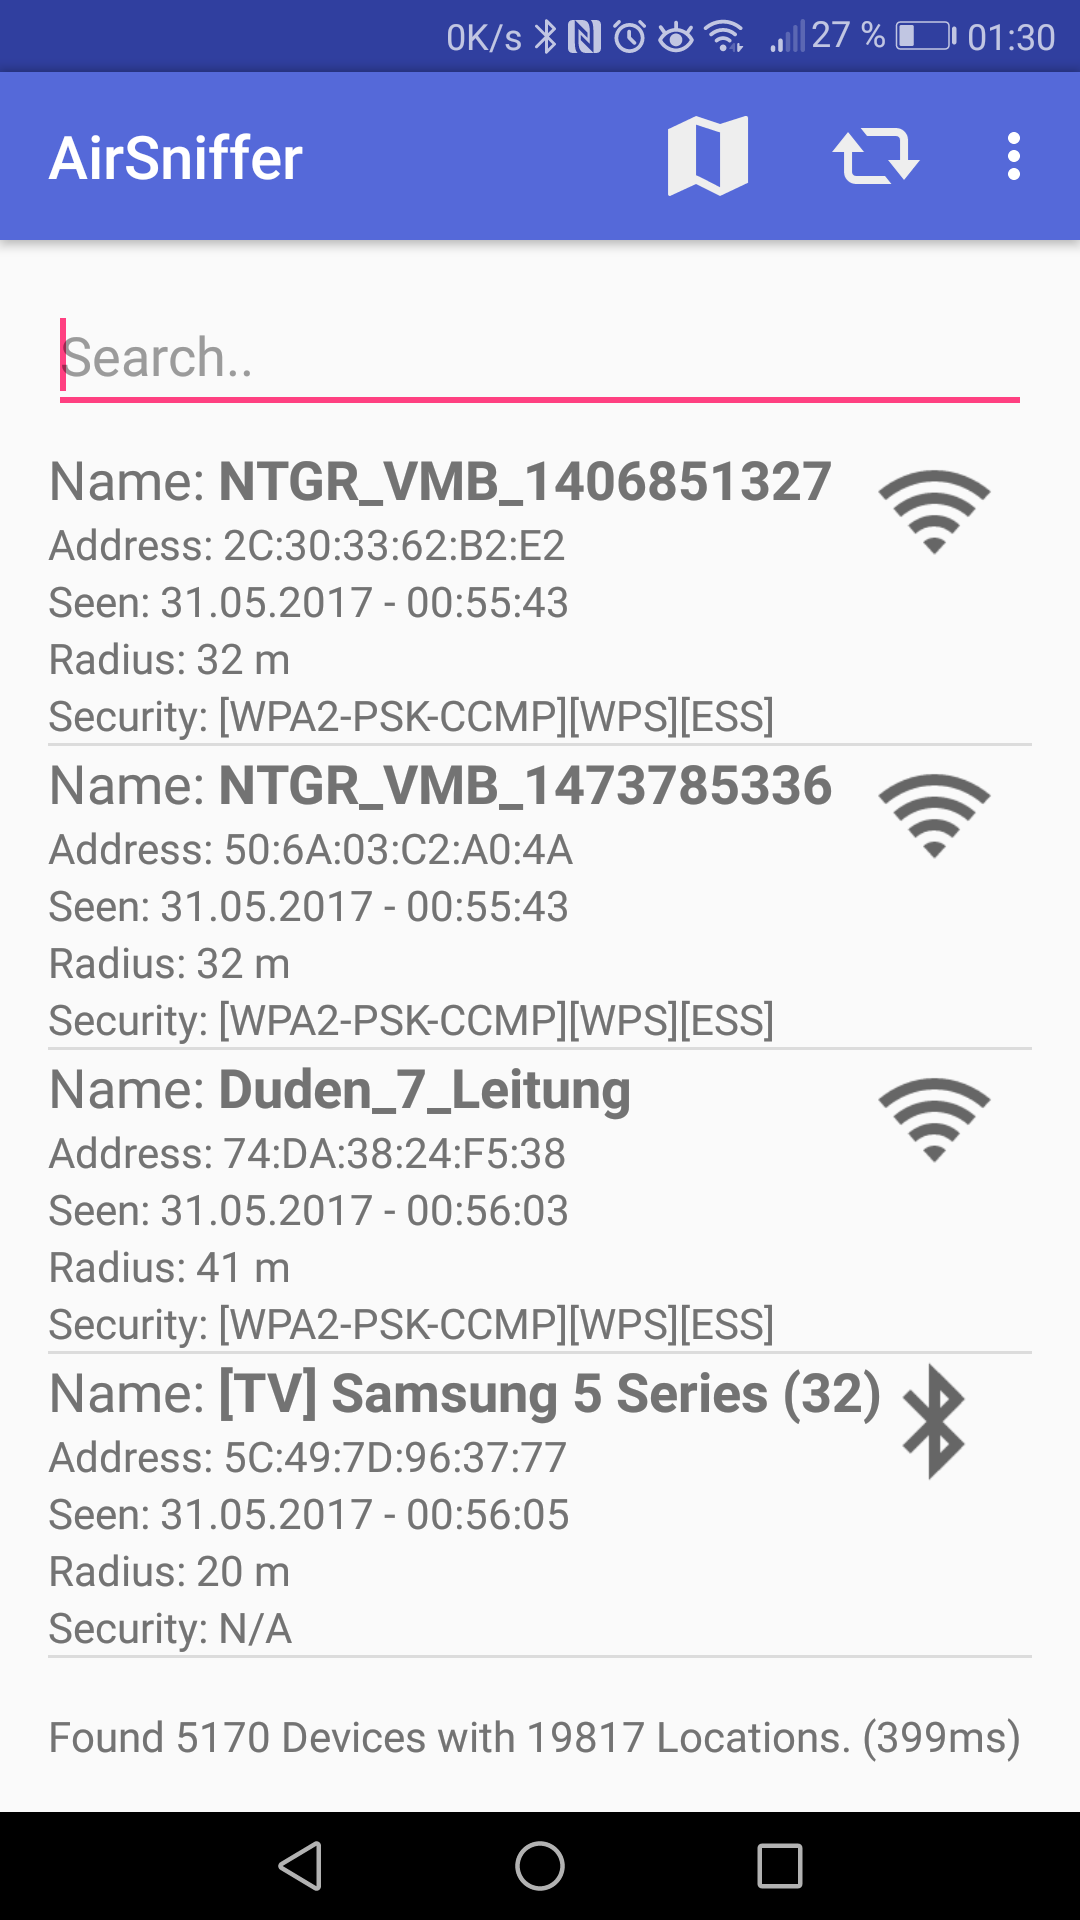
\includegraphics[width=\textwidth]{pics/screenshots/AirSniffer_Home_List.png}
        \caption{Homescreen mit allen gesehenen Geräten, Suchfunktion und Menü}
        \label{fig:AirSniffer_Home_List}
    \end{subfigure}
    \begin{subfigure}[htbp]{0.26\textwidth}
        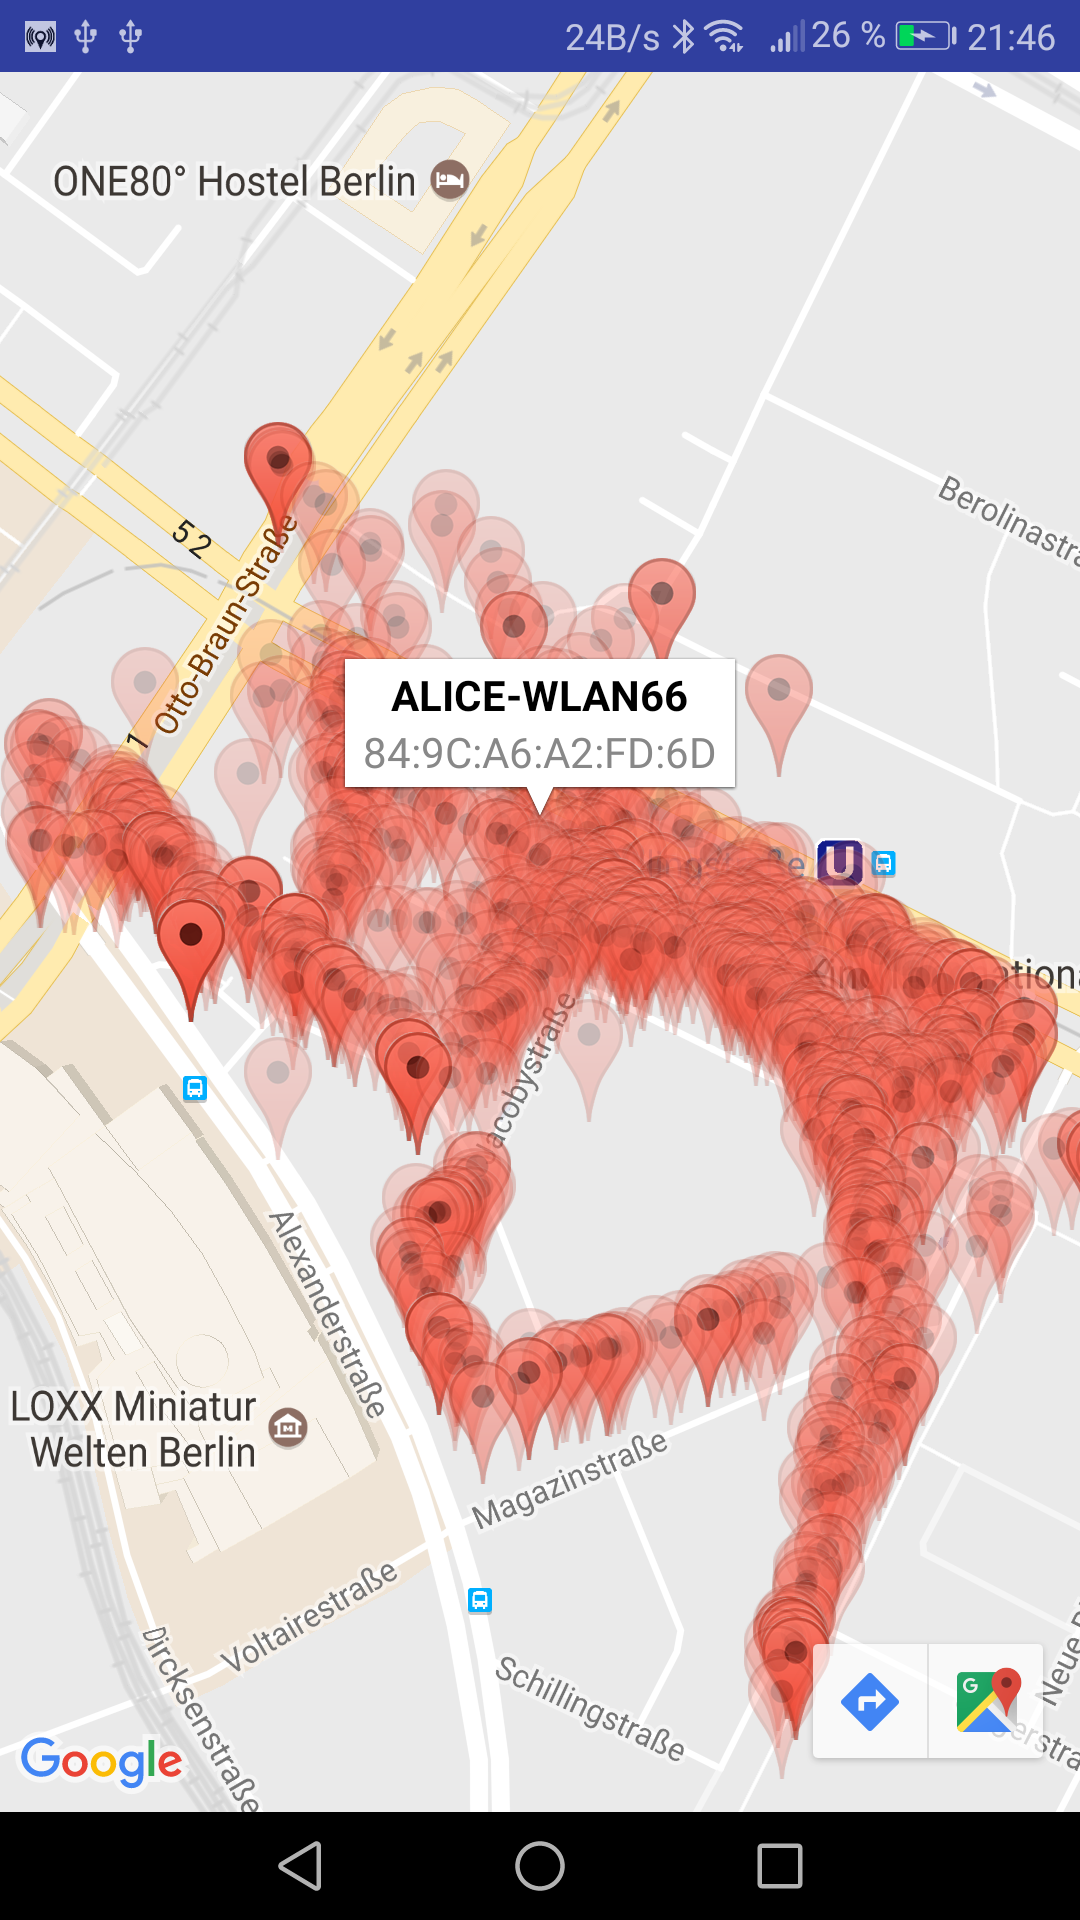
\includegraphics[width=\textwidth]{pics/screenshots/AirSniffer_Home_Map.png}
        \caption{Übersicht aller erfassten Geräte in einer interaktiven Karte}
        \label{fig:AirSniffer_Home_Map}
    \end{subfigure}
    \begin{subfigure}[htbp]{0.26\textwidth}
        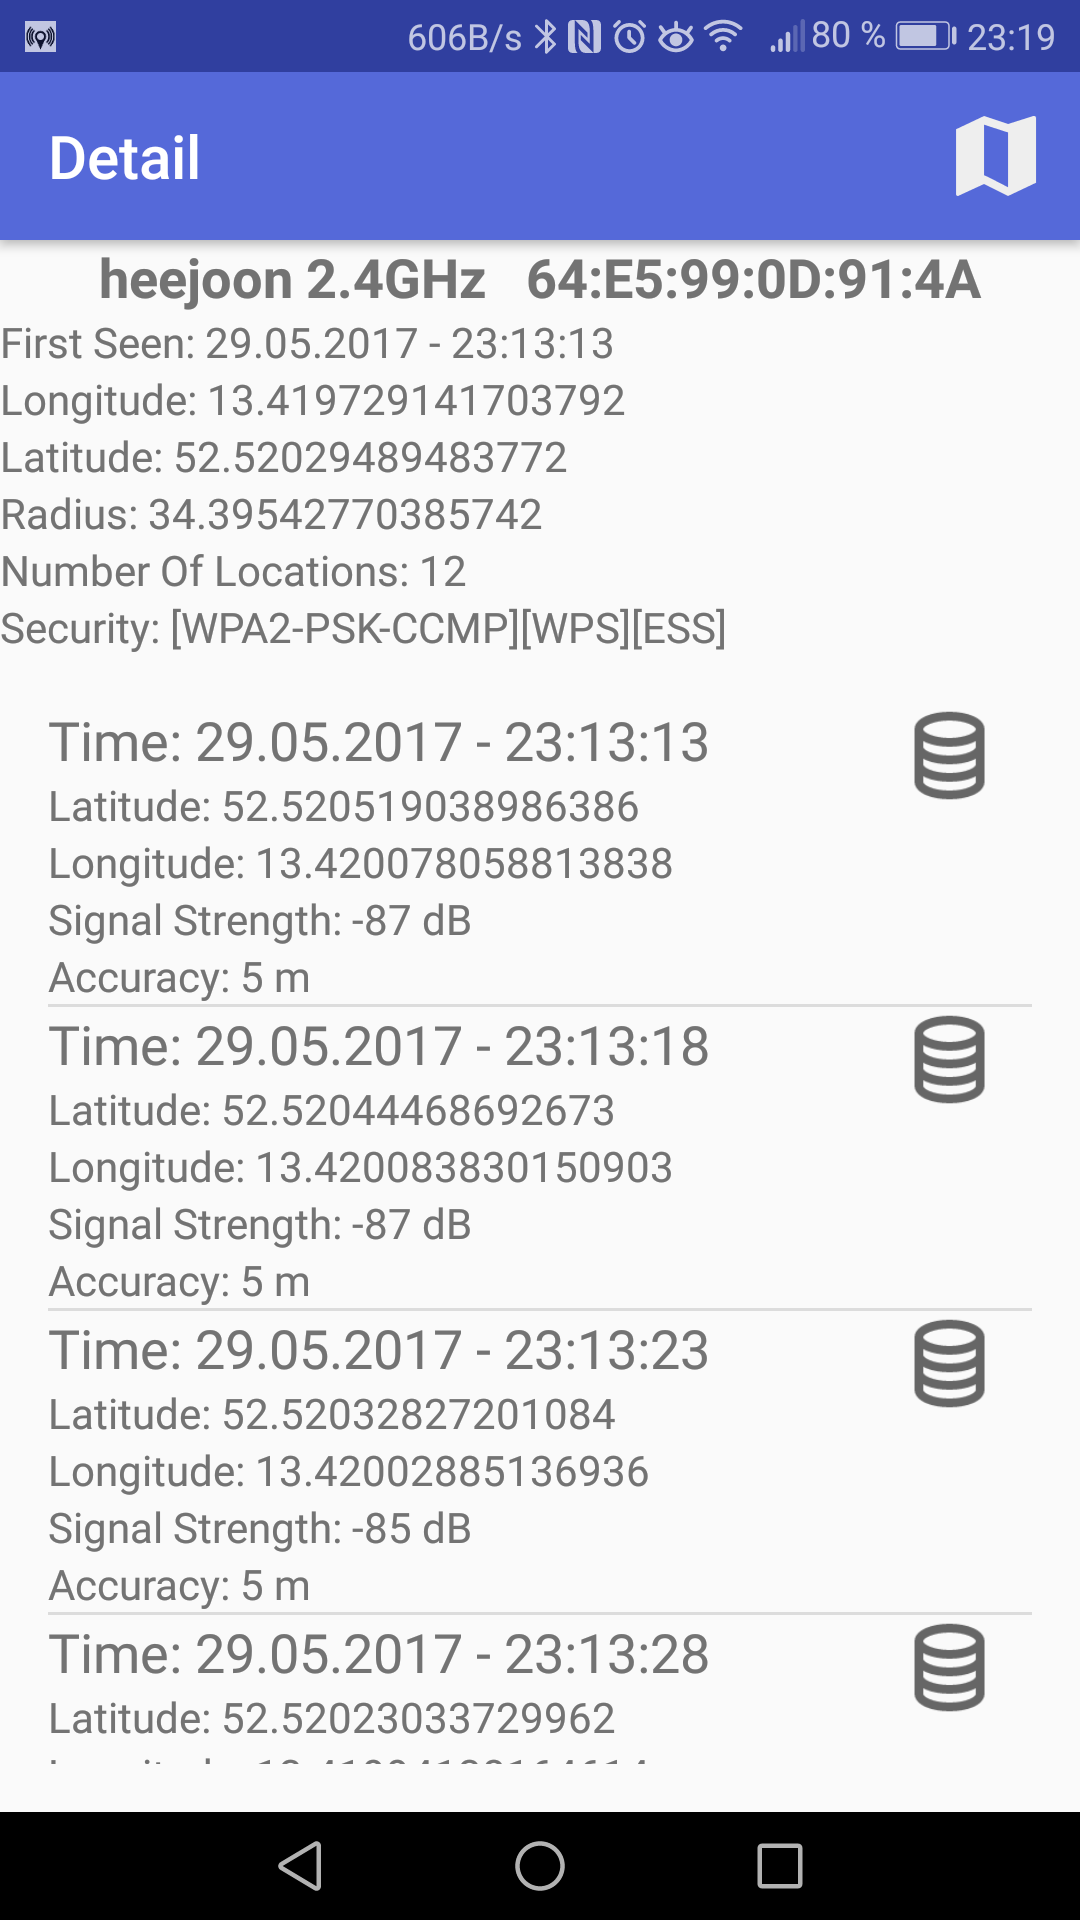
\includegraphics[width=\textwidth]{pics/screenshots/AirSniffer_Detail_List.png}
        \caption{Detailansicht eines Netzwerks inklusive aller zugehörigen Orte}
        \label{fig:AirSniffer_Detail_List}
    \end{subfigure}
    \begin{subfigure}[htbp]{0.26\textwidth}
        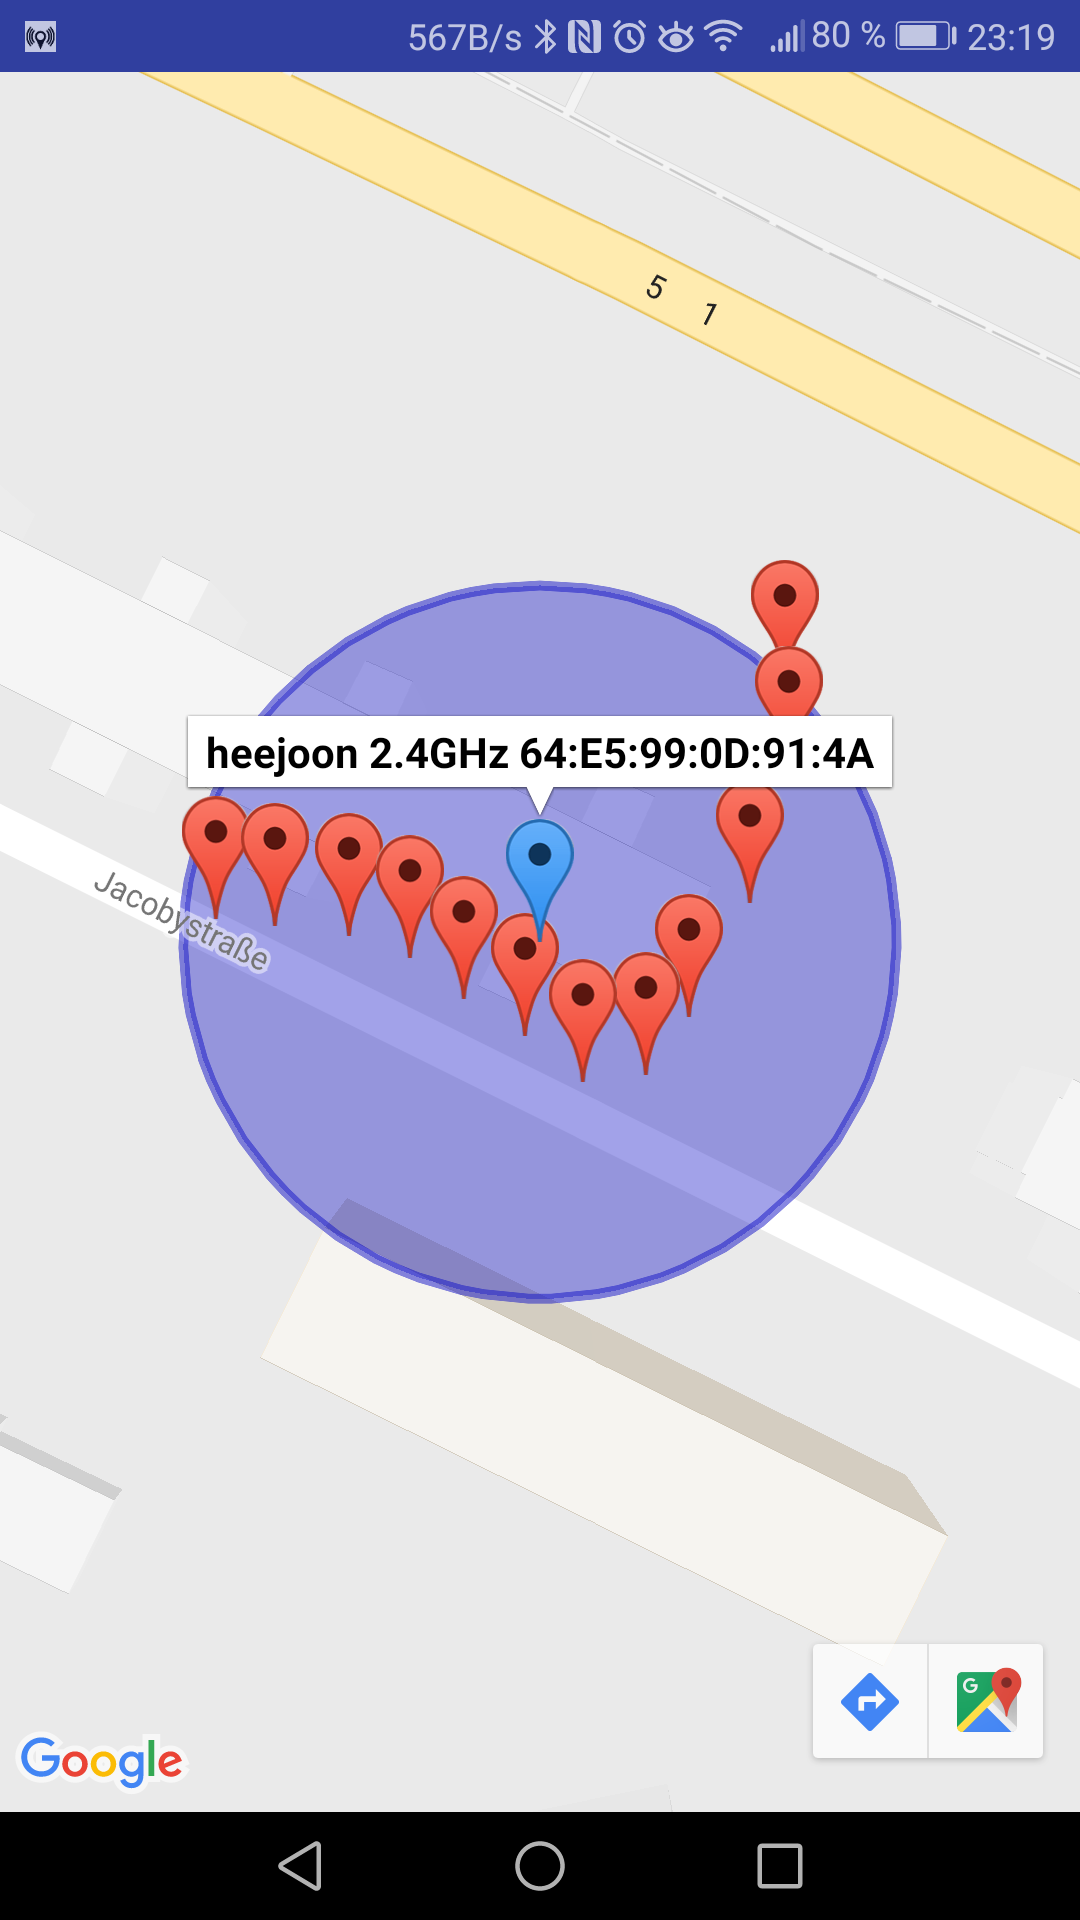
\includegraphics[width=\textwidth]{pics/screenshots/AirSniffer_Detail_Map.png}
        \caption{Detailansicht eines Netzwerks auf der Karte mit Anzeige der Ausbreitung}
        \label{fig:AirSniffer_Detail_Map}
    \end{subfigure}
    \begin{subfigure}[htbp]{0.26\textwidth}
        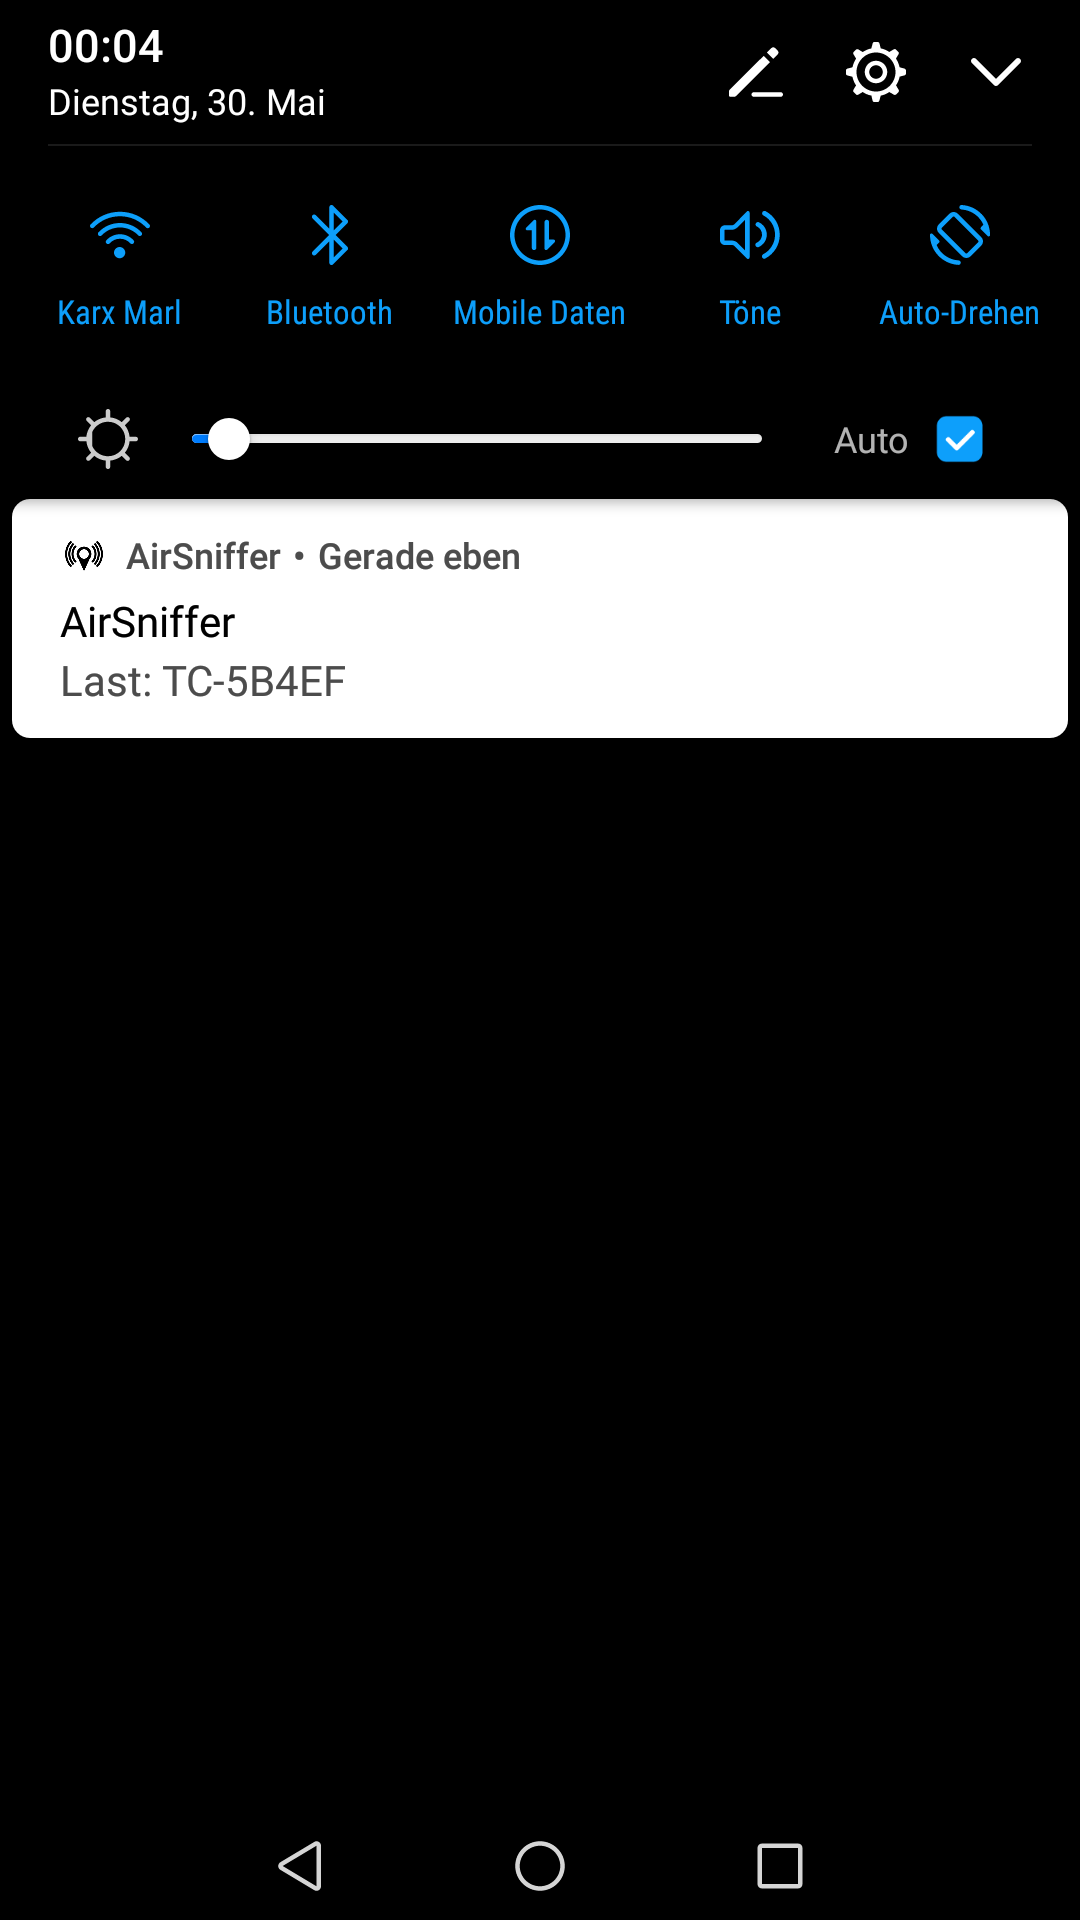
\includegraphics[width=\textwidth]{pics/screenshots/AirSniffer_Notification.png}
        \caption{Beispielhafte Benachrichtigung}
        \label{fig:AirSniffer_Notification}
    \end{subfigure}
    \begin{subfigure}[htbp]{0.26\textwidth}
        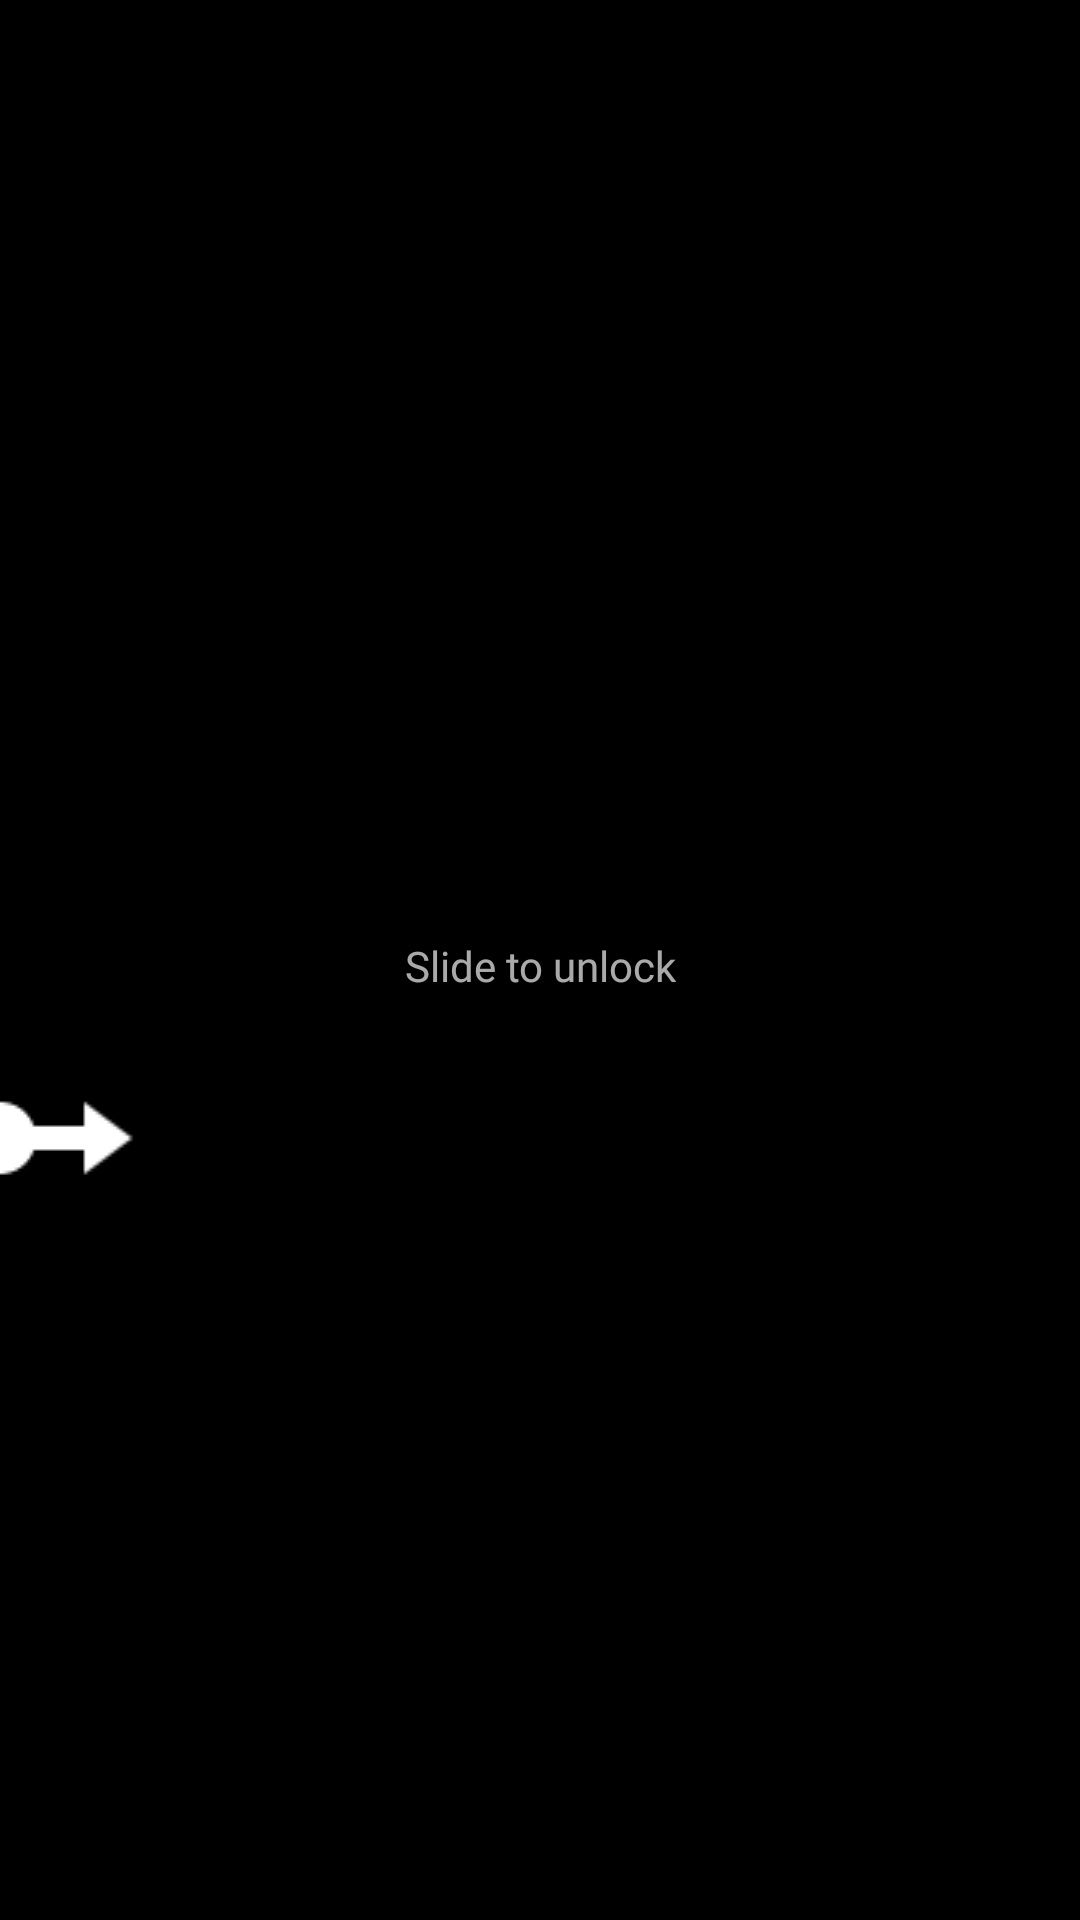
\includegraphics[width=\textwidth]{pics/screenshots/AirSniffer_Lockscreen.png}
        \caption{Sperrbildschirm}
        \label{fig:AirSniffer_Lockscreen}
    \end{subfigure}

    \caption{Screenshots der Smartphone App "AirSniffer}
    \label{fig:ScreenShots_AirSniffer}
\end{figure}

\newpage
\begin{figure}[htbp]
    \centering
    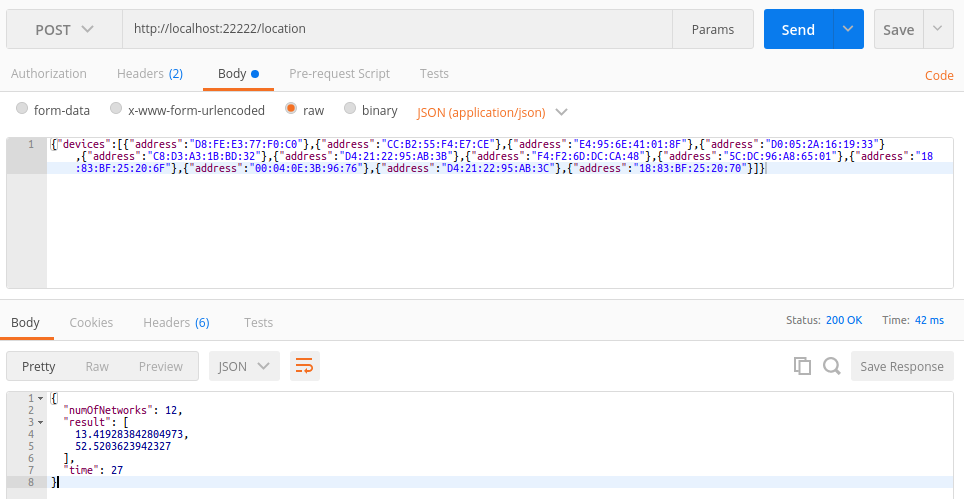
\includegraphics[width=0.92\textwidth]{pics/screenshots/AirPI_Request.png}
    \caption{API Request und Response an die "AirPI" für die Bestimmung der Position anhand von WLAN Daten}
    \label{fig:ScreenShot_AirPI}
\end{figure}

\begin{figure}[htbp]
    \centering
    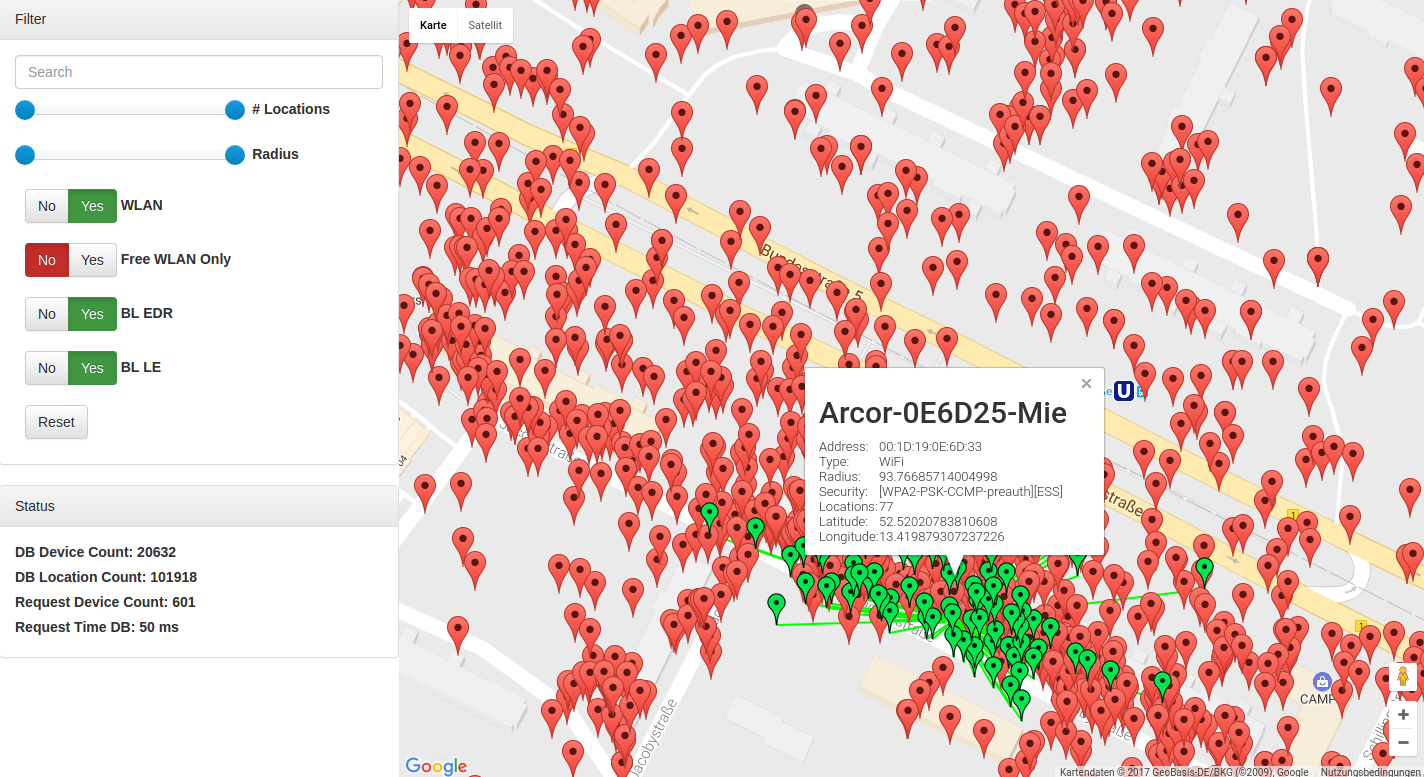
\includegraphics[width=0.92\textwidth]{pics/screenshots/AirVis.png}
    \caption{Oberfläche des Visualisierungstool "AirVis"}
    \label{fig:ScreenShot_AirVis}
\end{figure}

\newpage

\begin{figure}[htbp]
    \centering
        \begin{subfigure}[htbp]{0.38\textwidth}
        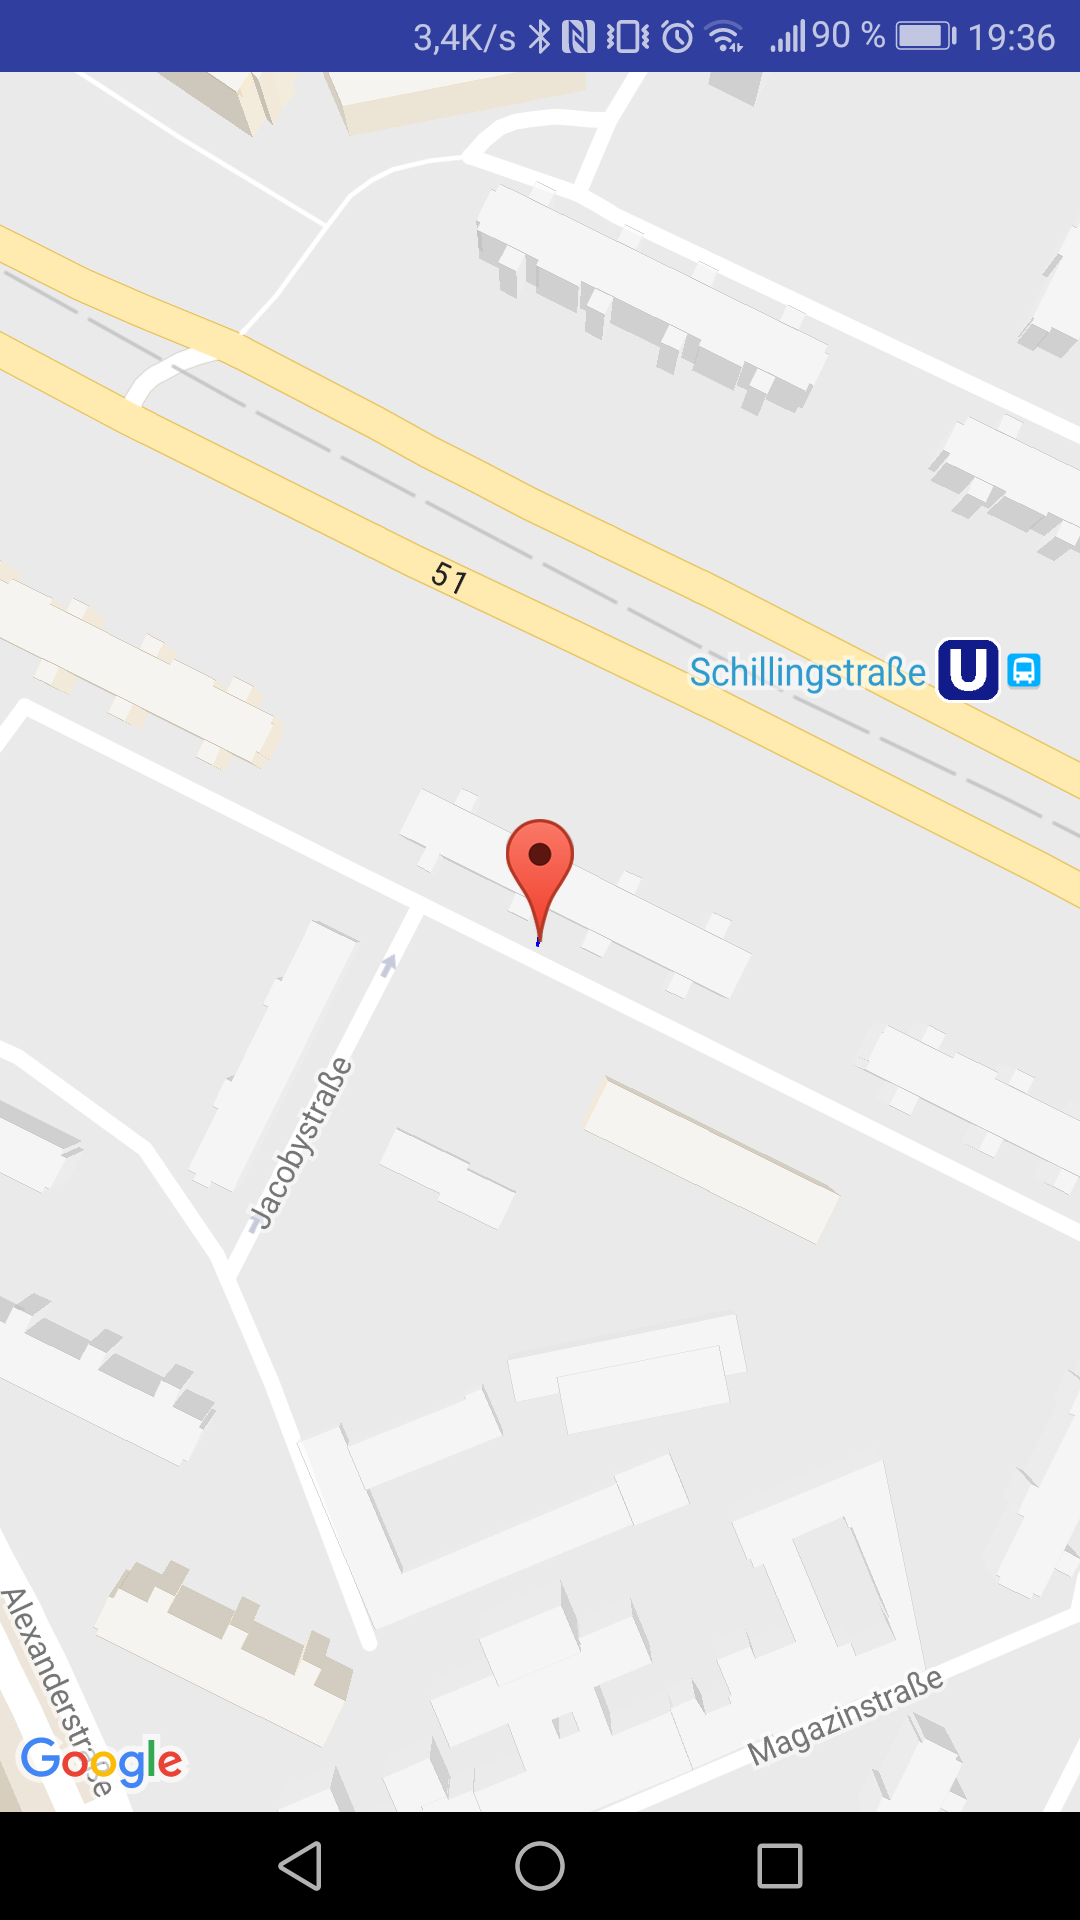
\includegraphics[width=\textwidth]{pics/screenshots/AirLocator_Single_Pos.png}
        \caption{Positionsbestimmung mittels des "AirLocator"}
        \label{fig:AirLocator_Single_Pos}
    \end{subfigure}
    \begin{subfigure}[htbp]{0.38\textwidth}
        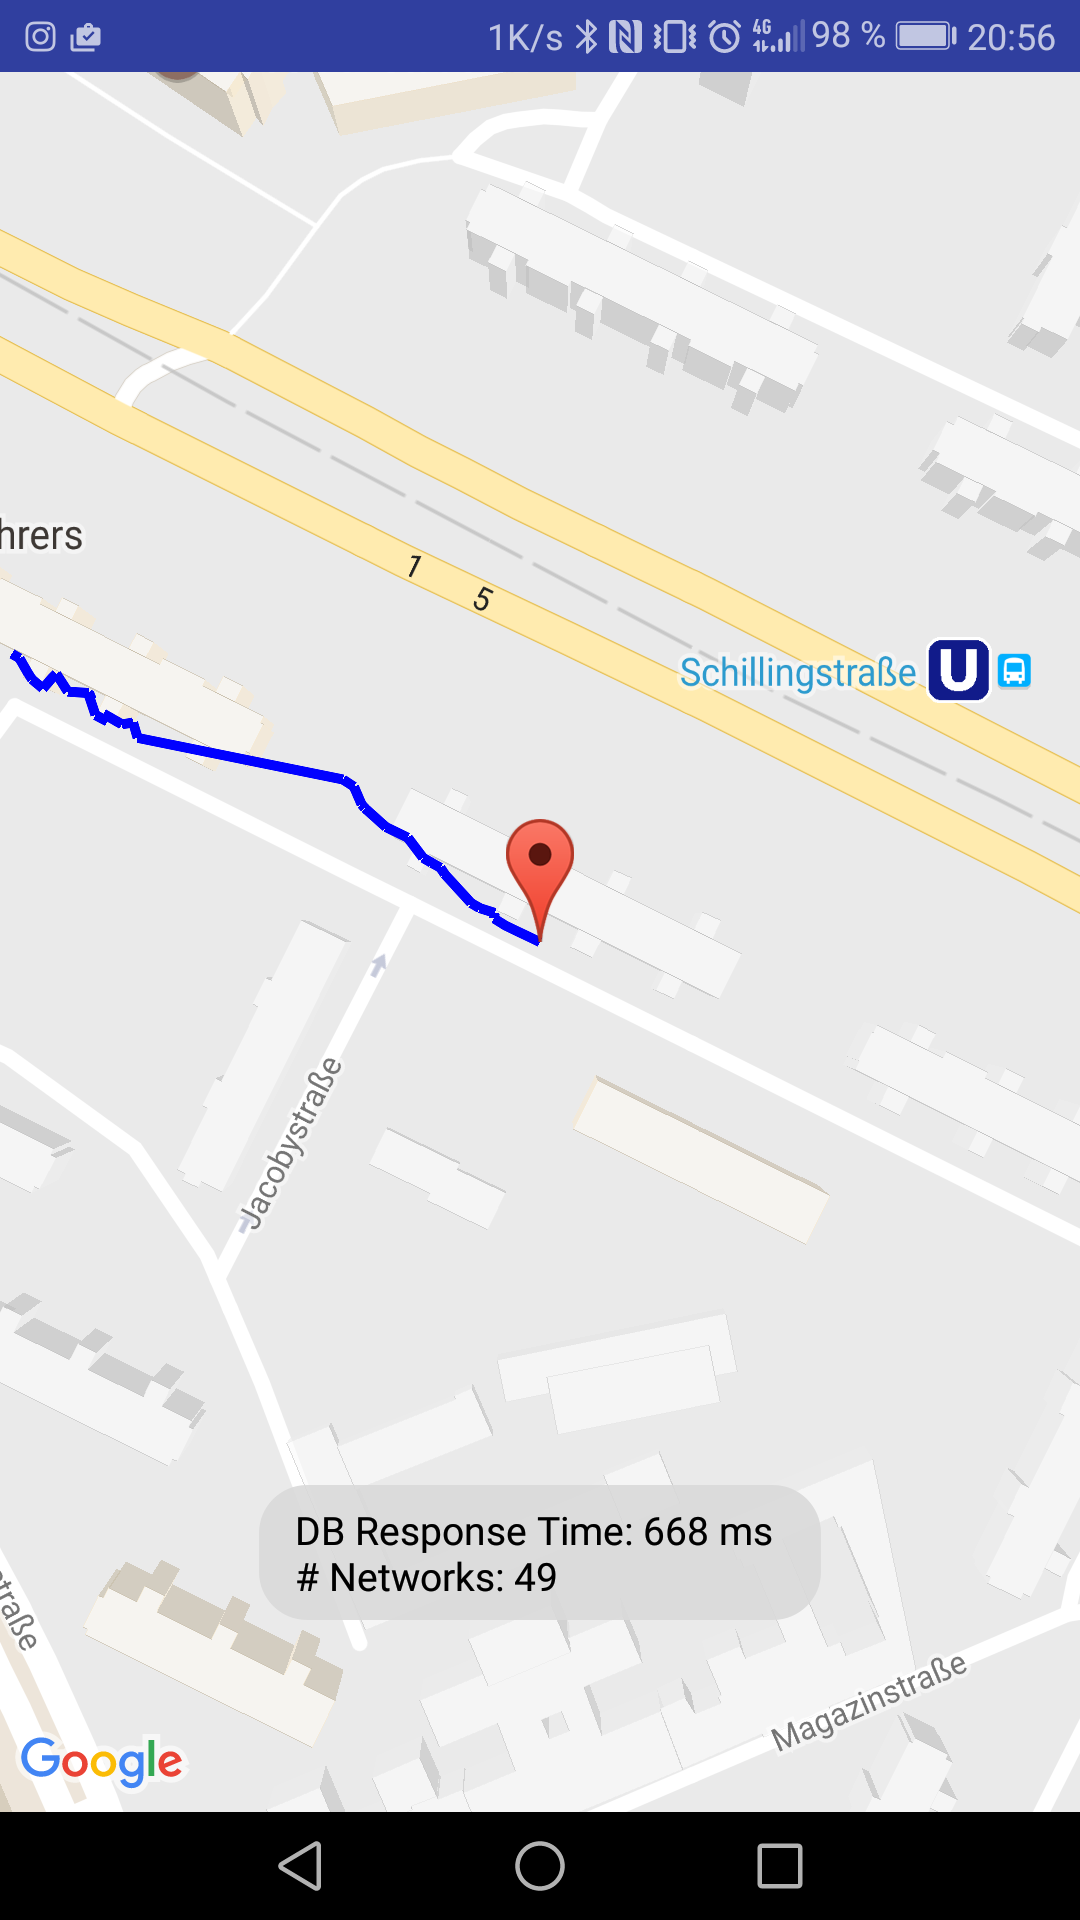
\includegraphics[width=\textwidth]{pics/screenshots/AirLocator_Multi_Pos.png}
        \caption{Verlauf der Positionsbestimmungen des "AirLocator" (gekennzeichnet mit blauen Pfad)}
        \label{fig:AirLocator_Multi_Pos}
    \end{subfigure}
    \caption{Screenshots der Smartphone App "AirLocator}
    \label{fig:ScreenShots_AirLocator}
\end{figure}


\newpage
\section{Abkürzungsverzeichnis}

\begin{acronym}
\acro{API}		{Application Programming Interface}
\acro{BL EDR}	{Bluetooth Enhanced Data Rate (Bluetooth 2)} 
\acro{BL LE}	{Bluetooth Low Energy (Bluetooth 4)}
\acro{GPS}		{Global Positioning System}
\acro{GUI}		{Graphical User Interface }
\acro{HTTP}		{Hypertext Transfer Protocol}
\acro{JSON}		{JavaScript Object Notation}
\acro{REST}		{Representational State Transfer}
\acro{SDK}		{Software Development Kit}
\acro{WLAN}		{Wireless Local Area Network}
\acro{WSGI}		{Web Server Gateway Interface}

\end{acronym}

\newpage
\begin{thebibliography}{99}

\bibitem{github} Github - Air Repository, https://github.com/fabiberlin/Air

\bibitem{gps} Official U.S. government information about the Global Positioning System (GPS) and related topics, http://www.gps.gov/systems/gps/

\bibitem{gpsfix} Wikipedia - Time to first fix, https://en.wikipedia.org/wiki/Time\textunderscore to\textunderscore first\textunderscore fix

\bibitem{skyhook} Skyhook - WiFi Location Based Marketing \& Tracking, http://www.skyhookwireless.com/

\bibitem{google_pos} Andorid SDK - Location Strategies, https://developer.android.com/guide/topics/location/strategies.html

\bibitem{wigle} Wigle - Wireless Network Mapping, https://www.wigle.net/

\bibitem{openwifi} OpenWifi.su - Open WLAN Map, http://openwifi.su/

\bibitem{googlemapsapi} Google Maps API, https://developers.google.com/maps/

\bibitem{sqlite} SQLite Dokumentation, https://sqlite.org/index.html

\bibitem{unlock_slider} Stack Overflow - Wow to make slide to unlock button in Android, https://stackoverflow.com/questions/14910226

\bibitem{harversine_distance} Harversine Distanz, 
https://rosettacode.org/wiki/Haversine\textunderscore formula

\bibitem{flask} Flask - Python Microframework,  http://flask.pocoo.org/

\bibitem{mongodb} MongoDB - Offical Website, https://www.mongodb.com/

\bibitem{pymongo} PyMongo Dokumentation, https://api.mongodb.com/python/current/

\bibitem{pine64} Pine64 Product Website, https://www.pine64.org/?product=pine-a64-board-2gb

\bibitem{sharding} MongoDB Sharding https://docs.mongodb.com/manual/sharding/

%TODO ICONS 8

\end{thebibliography}


\end{document}
